\ifdefined\included
\else
\documentclass[a4paper,11pt,twoside]{StyleThese}
\include{formatAndDefs}
\sloppy
\begin{document}
\setcounter{chapter}{2} %% Num�ro du chapitre pr�c�dent ;)
\dominitoc
\dominilof
\faketableofcontents
\fakelistoffigures
\fi

%%%%%%%%%%%%%%%%%%%%%%%%%%%%%%%%%%%%%%%%%%%%%%%%%%%%%%%%%%%%%%%%%%%%%%%%%%%%%%%%
\chapter{Pulling a hose}
\label{chap:hose}

\ifdefined\included
\else
\minitoc
\minilof
\fi

\cleardoublepage

From this chapter on we will present technical applications implemented on the real HRP-2.
This chapter discusses a strategy for a humanoid robot to pull a fire hose while walking towards a desired position and orientation. % of the robot. % on an unperfectly flat floor.
%
This work has been submitted to \emph{Humanoids} 2016.
%
In this chapter the motion planning for picking the fire hose from the floor is firstly presented.
%
Then a hybrid controller on the robot's wrist holding the fire hose is implemented for pulling it.
%
The proposed controller can automatically determine the pulling force according to the robot's walking velocity.
%
Through simulation analysis it is shown that when the robot walks while pulling the fire hose a drift in the walking direction is generated.
%
To cope with this drift and to direct the robot to a desired position and orientation, a walking task is introduced.
%
Using a motion capture system, the robot's chest position and orientation is monitored and feed to the robot's walking pattern generator to correct the orientation drift and to determine where to walk and when to stop walking.
%
Through experimental results the validity of the proposed strategy was confirmed.
%
It is shown that the proposed hybrid controller contributes to the improvement of the robot's balance when walking.
%
The video of the application can be found at \url{https://youtu.be/K33d2VTHTTA}

%%%%%%%%%%%%%%%%%%%%%%%%%%%%%%%%%%%%%%%%%%%%%%%%%%%%%%%%%%%%%%%%%%%%%%%%%%%%%%%%
\section{Motivation}    \label{sec_pick}
    %
After Japan's 2011 earthquake and Fukushima's nuclear power plant disaster, the importance of developing robots capable of helping/replacing humans in dangerous situations or with increased capabilities have raised quickly.
%
This natural disaster showed to the robotics community the lack of case studies that had been conducted towards applications in real case scenarios.
%
Having this as a motivation, in this work we focus on the task of pulling a fire hose by a humanoid robot.
%

Previous works on manipulation tasks by humanoid robots include pushing objects, pivoting, lifting, etc.
%
Hwang et~al. discussed whole body motions of a humanoid robot pushing a wall \cite{pushWall}.
%
Harada et~al. proposed a controller for pushing manipulation by a humanoid robot where the desired trajectory of the ZMP is modified to push an object \cite{pushingZMP}.
%
They also discussed planning the robot's gait in real time to push a heavy object \cite{pushRealTime}.
%
Takubo et~al. discussed pushing a heavy object by a humanoid robot.
The center of mass (CoM) trajectory is modified based on the forces acting on the robot's hands \cite{pushingChair}.
They also discussed a pushing method using multiple contact points between the robot and the object \cite{pushingChair2}.
%
Nozawa et~al. proposed a full-body motion controller for a humanoid robot to push a heavy object by considering the friction forces acting on the robot's arms \cite{pushingForceControl}.
%
Murooka et~al. proposed a whole-body pushing motion by a humanoid robot considering force and balance and using selected contact points with the object to be pushed \cite{pushDesk}.
%
%
Murooka et~al. also discussed the manipulation strategy to use for various objects by a humanoid robot.
The forces applied on the robot are known but not the object dynamical parameters.
Lifting, sliding and tilting the object are the three strategy that are taken into account \cite{Murooka:icra:2014}.
%
Harada et~al. discussed the task of lifting an object and then walk while holding it \cite{heavyObject}.
%

%
\begin{figure}[t]
 \centering
 \includegraphics[height=0.40\textwidth]{./figures/Hose_HRP2.pdf}
 \vspace{-3mm}
 \caption{The fire hose is empty and rolled up into a reel used in this work is shown in (a) and the humanoid robot HRP-$2$ is shown in (b).}
 \label{rob_hose}
% \vspace{-5mm}
\end{figure}


%As far as we know, there has been no work on manipulating a fire hose by a humanoid robot.
%
In this work, we discuss the task of picking and then pulling a real fire hose by a humanoid robot while it walks.
%
The fire hose is empty and rolled up into a reel that is fixed to the floor as shown in Fig.~\ref{rob_hose}(a) the nozzle of the hose lays on the floor.
%
A humanoid motion planner is used to generate the picking motion of the humanoid robot HRP-$2$ to avoid any self-collision when the robot leans forward to pick the hose.
%
Then a user friendly walking pattern generator, which input is a velocity relative to the ground plane, is used to generate the walking motion.
%
For pulling the hose a hybrid controller on the robot's wrist holding the hose was implemented.
%
Through simulation analysis it is shown that when the robot is walking while pulling the hose, a drift on the robot's walking direction is generated.
%
A walking task is introduced to correct this drift.
%
Using a motion capture system, the robot's chest position and orientation is tracked in real time.
%
The walking task will compute the desired reference velocity for the robot to arrive to a desired position/orientation.
%
Experimental results confirm the validity of the proposed motion for picking and pulling a fire hose.
%
Moreover we show that the hybrid controller contributes to the improvement of the robot's balance when walking.
%
It must be pointed out that whereas most of the previous work on pushing/pulling is based on force control, in this work we use a combination of position and force control to tackle the drift generated by the fire hose when the robot is walking.


This chapter is organized as follows: 
%
in section \ref{sec_pick} we present the motion planning for the robot to pick the fire hose from the floor.
%
In section \ref{sec_wpg} we briefly introduce the walking pattern generator used in this work.
% 
In section \ref{sec_pull} we show the strategy for a humanoid robot to pull a fire hose and analyze simulation results.
%
In section \ref{sec_wtask} we introduce a walking task to correct the drift in the robot's walking direction generated by the hose.
%
In section \ref{sec_exp} we show the experimental results of the proposed strategy using the HRP-$2$ humanoid robot.
%
Finally, in section \ref{sec_con} we give the conclusion of this work and briefly discuss future work.


\section{Picking motion}    \label{sec_pick}
    %\section{Humanoid Path Planner (HPP)}

The complex motion of leaning forward and picking the hose from the floor pose several problems.
%
First auto collisions are possible between the femurs and the hip joints due to the structure design of the HRP-$2$ humanoid robot.
%
Second a reactive approach does not find a good solution because of local minima.
%
For these reasons we employed the Humanoid Path Planner (HPP) to compute the motion for picking the hose from the floor.
%
This exact same versatile library we used to plan the contact point on the multi-contact climbing stair motion in Chap.~\ref{chap:multicontact}.
%
As a reminder HPP, \cite{hpp} is an open source software able to compute a collision-free path from a given starting robot configuration to a goal one.
%
This path is subject to a set of constraints such as balance conditions, a particular posture for specific DOF(s), etc.
%
It is also able to randomly search for a robot configuration satisfying a set of desired constraints, including environment and self-collision checking.
%
For picking the fire hose from the floor, first we search for a robot configuration with the following constraints:
%
\vspace{0.7mm}
\begin{list}{\arabic{ass}.}{%
		\usecounter{ass}%
		\setlength{\topsep}{2pt}%
		\setlength{\itemsep}{0pt}%
		\setlength{\parsep}{0pt}%
		\setlength{\labelwidth}{1.5em}%
		\setlength{\leftmargin}{1.5em}%
		\setlength{\labelsep}{0.5em}%
	}
%
\item The robot's center of mass must be at the center of the support polygon.
%
\item Both of the robot's feet should keep in contact with the floor.
%
\item The left wrist height must be such that it can reach the hose without colliding with the floor.
%
\item The robot's waist orientation is fixed and facing forward.
%
\end{list}


Furthermore, we use the robot's half sitting configuration to limit the results from the random search to configurations that satisfy:
%
\vspace{-1mm}
\begin{equation*}
\mathbf{q}_{\text{res}} = \mathbf{q}_{\text{rand}}' + \big( \mathbf{I}_{\text n} - \mathbf{J}^{+}\mathbf{J}(\mathbf{q}_{\text{rand}}')(\mathbf{q}_{\text{hs}} - \mathbf{q}_{\text{rand}}') \big)
\vspace{-1mm}
\end{equation*}
%
where $\mathbf{q}_{\text{rand}}'$ is the projection of a random configuration $\mathbf{q}_{\text{rand}}$ into the constrained space, $\mathbf{q}_{\text{hs}}$ is the robot's half sitting configuration, $\mathbf J$ is the Jacobian of the robot tasks and $\mathbf{I}_{\text n}$ is the identity matrix of $n\times n$, and $\mathbf{q}_{\text{res}}$ is the projection of $\mathbf{q}_{\text{hs}}$ on the constrained tangent space at $\mathbf{q}_{\text{rand}}'$.
%
The desired robot configuration is the projection of $\mathbf{q}_{\text{res}}$ into the constrained space $\mathbf{q}_{\text{res}}'$. 
%
%
After obtaining the picking configuration, we compute two free collision paths, the first starting at the half sitting configuration and finishing on $\mathbf{q}_{\text{res}}'$, and the second starting at $\mathbf{q}_{\text{res}}'$ and going back to the half sitting configuration, both of them subject to constraints 1, 2 and 4 during the whole path.
%
From the obtained path we extract the information of the robot's center of mass position, both feet's position and orientation, and the robot's configuration angles.
%
These information will be use by an inverse kinematic framework for redundant robots that prioritizes robot tasks by projecting low priority tasks into the kernel of high priority tasks \cite{mansard:icar:09}.
%
\begin{figure}[t]
 \centering
 \includegraphics[height=0.40\textwidth]{./figures/Pick_2pics.pdf}
 \vspace{-3mm}
 \caption{Snapshots of the experiment on the HRP-$2$ robot picking a fire hose from the floor.}
 \label{exp_pick}
% \vspace{-5mm}
\end{figure}


\section{The walking pattern generator} \label{sec_wpg}
    In order to control the displacement of the humanoid robot HRP-$2$ we used the walking pattern generator presented in Chap.~\ref{chap:nmpc} and published in \cite{naveau:ral:2016}.
As a reminder, this walking pattern generator allows the user to control a humanoid robot almost like a mobile platform.
The input of the walking pattern generator is a velocity $ [\dot{x},\dot{y},\dot{\theta}] $ relative to the ground plane, and is tracked by the center of mass.
The walking pattern generator computes automatically the foot transitions and the center of mass trajectory, so that the robot is balanced when walking.

In this walking pattern generator, the input velocity is tracked by the center of mass if all the constraints are respected.
As a consequence the walking pattern generator will create a swinging motion of the center of mass from one foot to the other even if the input velocity is zero on the robot coronal plane.
The robot will move its center of mass to maintain balance while walking in any circumstances.
%This particular behavior causes perturbations in control laws during the localization of the robot.
%In practice the goal position is set as zone where the CoM has to fitin and 
This swinging motion has to be taken into account when designing the hand tasks to avoid auto-collision and the walking task to make the robot converge toward a specific goal.



\section{Pulling strategy}		\label{sec_pull}
		In this section we explain the strategy for pulling the fire hose while walking.
%
First, we described the hybrid controller used to control the robot's wrist holding the hose.
%
Then, simulation results are shown for analyzing and demonstrating the robot's behavior when pulling the fire hose while walking.





\subsection{Hybrid controller}			\label{pulling}

\begin{figure}[ht]
 \centering
 \includegraphics[height=0.40\textwidth]{./figures/coordinates.pdf}
 \vspace{-4mm}
 \caption{The robot coordinate frame.}
 \label{frame}
% \vspace{-5mm}
\end{figure}
%
In order to pull the fire hose while walking a hybrid controller is implemented on the robot's wrist holding the hose.
%
Position control is employed to keep a fix distance between the waist of the robot and it's wrist, and impedance control is employed to pull the hose.
%
According to the frame attached to the robot (as shown in Fig.~\ref{frame}), position control is used in $Y$ direction and impedance control in $X$ and $Z$ directions.
%
%
%
%
% 
%
The impedance controller on the left wrist is defined similarly to the one proposed by Harada et~al. \cite{pushRealTime} as:  
%
\begin{equation}
m\mathbf{\ddot{x}}_{lw} + c\mathbf{\dot{x}}_{lw} = \mathbf{f}_{lw} - \mathbf{f}_d - \mathbf{f}_{\text{pull}} \; ,
\label{eq_imp}
\end{equation}
%
where $\mathbf{x}_{lw} = [x_{lw} \; y_{lw} \; z_{lw}]^T$ represents the robot's left wrist position, and $m$ and $c$ are the desired mass and damping coefficients, respectively.
%
The force applied to the left wrist of the robot is represented by $\mathbf{f}_{lw}$, $\mathbf{f}_d$ is the desired force in the left wrist, and $\mathbf{f}_{\text{pull}}$ represents the desired pulling force, defined as:
%
%
\begin{equation}
\mathbf{f}_{\mathrm{pull}} = \begin{cases}
\mathbf{W} \mathbf{v}^{\mathrm{ref}}	& \quad \mathrm{if} \; z_{la} = z_{ra} = h_a  \\
0  & \quad \mathrm{otherwise} \\
\end{cases}
, 
\label{fpull}
\end{equation}
%
where $z_{la}$ and $z_{ra}$ are the $Z$ direction components of the left and right ankles, $h_a$ is the height of the ankles when making full contact with the floor, $\mathbf{v}^{\text{ref}}$ is the reference velocity vector of the robot when walking and $\mathbf{W}$ is a diagonal matrix.
%
Like this, the robot will pull the hose only at the double support phase when walking and will not pull the hose when standing still.
%
Furthermore, the diagonal matrix $\mathbf{W}$ allows to select in which direction to pull the hose.


The orientation of the wrist will be kept constant with respect to the orientation of the robot's waist, i.e. it will rotate in the same direction, same amount as the robot's waist.


\subsection{Simulation analysis}			\label{sim_pulling}
%
%
\begin{figure}[ht]
 \centering
 \includegraphics[height=0.40\textwidth]{./figures/yaw_drift_simGraph.pdf}
 \vspace{-3mm}
 \caption{Snapshots of the top view of the simulation of HRP-$2$ robot holding a hose in (a) to (c), and the change in the robot's yaw angle in (d).}
 \label{drift_sim}
% \vspace{-5mm}
\end{figure}
%
%
The humanoid robot HRP-$2$ is simulated using the OpenHRP software version 3.1.2.
This software simulates the dynamics of the hose and HRP-$2$ during the walk.
%
To generate the walking motion of the robot the walking pattern generator described in section \ref{sec_wpg} is used.
%
The fire hose is approximated by a simplified model consisting of rigid cylinders connected by rotational joints with the rotation axis parallel to the cross section of the cylinders.
%

Fig.~\ref{drift_sim} shows the simulation results of the yaw orientation angle of the robot's waist when using a fire hose with a length of $7$ m partially rolled up at the starting time (Fig.~\ref{drift_sim}(a)).
%
The hose has a total mass of $13.2$ kg, which includes the mass of the nozzle and the coupling of the hose.
%
A uniform mass distribution of $1.8$ kg/m, which correspond to the real fire hose, is assumed for the cylinders.
%
The reference velocity given to the pattern generator is $\mathbf v_{\text ref} = [0.1 \; 0.0 \; 0.0]^T$ and it is constant through all the simulation.
%
As it can be seen in Fig.~\ref{drift_sim}, after walking few steps the robot begins to drift to its left with an almost constant velocity.
%
It can be inferred that the force generated by the hose on the robot's wrist generates a slip on the robot's feet, thus generating a drift in the robot's yaw angle.
%


Furthermore, it was discovered that the amount of drift depends on the mass of the fire hose.
%
The change in the yaw angle in simulation using hoses with different weights is shown in Fig.~\ref{drift_sim2}.
%
The light, normal an heavy hoses have a total mass of $4.52$, $9.04$ and $13.56$ kg, respectively and a length of $1.8$ m for each of them.
%
From this results it can be observed that the drift on the orientation of the robot depends on the disturbance given by pulling the hose on its left wrist.
%
%
\begin{figure}[t]
 \centering
 \includegraphics[height=0.3\textwidth]{./figures/yaw_drifts_3weights.pdf}
 \vspace{-3mm}
 \caption{Change in the robot's yaw angle for three different weights per length unit. Light's hose mass is $4.52$ kg, normal's hose mass is $9.04$ kg and heavy's mass is $13.56$ kg}
 \label{drift_sim2}
% \vspace{-5mm}
\end{figure}




\section{Walking task}          \label{sec_wtask}
		In this section we introduced  a walking task to deal with the drift generated on the yaw angle of the robot when walking while holding the fire hose, as explained in the previous section.
%
Then, simulation results are shown to confirm the validity of the proposed walking task.



To cope with the drift in the walking direction explained in the previous section, we introduced a walking task $\mathbf{e}_w$ which is defined as:
%
\begin{equation}
\mathbf{e}_w = \mathbf{x} - \mathbf{x}_d \; ,
\label{ewalk}
\end{equation}
%
where vector $\mathbf{x} = [x_c \; y_c \; \phi_c]^T$ includes the robot's chest $X$ and $Y$ direction position and its yaw orientation angle $\phi$. Similarly, the desired position and yaw angle is represented by $\mathbf{x}_d$.
%
Therefore, the desired reference velocity for walking $\mathbf{v}^{\text{ref}}$ is obtained as:
%
\begin{equation}
\mathbf{v}^{\text{ref}} = -\lambda \mathbf{e}_{w} - \mathbf{\Lambda} \int \mathbf{e}_{w}(t)  \; \mathrm{d}t \; ,
\label{velwalk}
\end{equation}
%
where $\lambda$ is an adaptive gain and the matrix $\mathbf{\Lambda}$ is a diagonal matrix of adaptive gains. 
%
The obtained reference velocity is used as an input to the walking pattern generator that will calculate the footsteps of the robot in real time, and also as an input to the impedance controller that will compute the desired pulling force according to the robot's reference velocity.
%
Fig.~\ref{sim_graph} shows the simulation results for a walking task with $\mathbf{x}_d = [4.0 \; 0.0 \; 0.0]^T$ when the robot starting position is $\mathbf{x}_i = [0.0 \; 0.0 \; 0.0]^T$.
%
A maximal velocity of $0.10$ and $0.15$ m/step for the $X$ and $Y$ directions, respectively, and $5$ deg/step are set to the walking task.
%
%
\begin{figure}[t]
 \centering
 \includegraphics[height=0.40\textwidth]{./figures/sim_pos.pdf}
 \vspace{-3mm}
 \caption{Robot's waist trajectory in simulation. In (a) position in $X$ direction, in (b) position in $Y$ direction and in (c) yaw angle.}
 \label{sim_graph}
% \vspace{-5mm}
\end{figure}
%
%
It can be seen that the robot reaches the desired position within $80$ seconds and also that the walking task is able to correct the drift generated by the hose.

         
\section{Experimental results}		\label{sec_exp}
		%
\begin{figure*}
  \centering
  %!TEX root = ../../14-icra-RealTimeNMPC.tex

\tikzstyle{block} = [draw, fill=blue!20, rectangle,
    minimum height=2em, minimum width=5em, align=center]
\tikzstyle{sum} = [draw, fill=blue!20, circle, node distance=1cm]
\tikzstyle{input} = [coordinate]
\tikzstyle{output} = [coordinate]
\tikzstyle{pinstyle} = [pin edge={to-,thin,black}]

% The block diagram code is probably more verbose than necessary
\begin{tikzpicture}[auto, node distance=2cm,>=latex]
    % We start by placing the blocks
    \node [input]  at (-1.5, 0.0) (input)  {};
    \node [input]  at (-0.5, -1.0) (feedback)  {};
    \node []    at ( 0.0, 0.0) (sumin)  {};
    \node [output]    at ( 14, 0.0) (sumout) {};

    \node [block] at (0.8,0) (wpg) {
        Walking\\
        Pattern\\
        Generator
    };
    \node [block] at (3.8,0) (dyn) {
        Dynamic\\
        Filter
    };
    \node [block] at (7.0,0) (sot) {
        Generalized\\
        Inverse\\
        Kinematics
    };
    \node [block] at (10.5, 0) (system) {
    		Robot Hardware\\
    		{\small Simulation/Robot}
    	};

    % PATHS
    	% Forward chaine
    \draw [draw,->] (input) -- node {\small ${Vel}^{\,ref}$} (wpg);
    \draw [draw,->] (wpg) -- node [text width=0.7cm]{\small $c^{ref}$ $f^{ref}$} (dyn);
    \draw [draw,->] (dyn.east) -- node [text width=0.7cm]{\small $\tilde{c}^{\,ref}$ $f^{ref}$} (sot);
    \draw [draw,->] (sot) -- node [text width=0.7cm]{\small $q^{ref}$ $\dot q^{ref}$} (system);
    %\draw [->] (system) -- node {} (sumout);

    % Feedback chaine
    \draw [- ] ($(dyn.east) + (0.35,0.0)$)  |- node {} (feedback);
    \draw [->] (feedback) |- node {} ([yshift=-0.2cm]wpg);

%    \draw [->] (dyn) -| node[above right] {\small $\hat{c}^{\,x,y,\theta}$, $\hat{f}^{\,\,x,y,\theta}$} (wpg);
\end{tikzpicture}


% The block diagram code is probably more verbose than necessary
%\begin{tikzpicture}[auto, node distance=2cm,>=latex']
%    % We start by placing the blocks
%    \node [input]  at (-0.5, 0.0) (input)  {};
%    \node [sum]    at ( 0.5, 0.0) (sumin)  {};
%    \node [sum]    at ( 6.5, 0.0) (sumout) {};
%    \node [output] at ( 7.5, 0.0) (output) {};
%
%    % QP Controller Blocks
%    \node [block] at (2.0,0) (oriqp) {
%        QP Controller\\
%        \small{Orientation}
%    };
%    \node [block] at (5.0,0) (posqp) {
%        QP Controller\\
%        \small{Position}
%    };
%    \node [block] at (5.0, -2.0) (dynamics) {Dynamics};
%    \node [block] at (2.0, -2.0) (system)   {System};
%
%    % PATHS
%    \draw [draw,->] (input) -- node {$
%        \dot C_{k+1}^{ref}
%    $} (sumin);
%    \draw [->] (oriqp) -- node {$U_k$} (posqp);
%    \draw [->] (posqp) -- node {$U_k$} (sumout);
%    \draw [->] (dynamics) --  (system);
%
%    \draw [->] (sumout) -- node {$ $} (output);
%    \draw [->] (sumin) -- node {} (oriqp);
%    \draw [->] (sumout) |- node[near start] {$y$}   (dynamics);
%    \draw [->] (system) -| node[near end]   {$val$} (sumin);
%\end{tikzpicture}

 \vspace{-3mm}
 \label{feed_back_graph}
\end{figure*}
%

%In this section the experimental results of the picking motion explained in section \ref{sec_pick} and the proposed strategy for pulling a fire hose with the HRP-$2$ humanoid robot are presented.


In Fig.~\ref{feed_back_graph}, the feedback control loop used in the experiments is shown.
%
The walking task uses the robot's chest position given by the motion capture system to compute the reference velocity $\mathbf{v}_{\text{ref}}$ for the walking pattern generator.
%
$\mathbf{v}_{\text{ref}}$ is also used by the impedance controller to compute the pulling force to be applied.
%
The reference positions for the feet and the center of mass are computed by the walking pattern generator, and the reference position of the left wrist is computed by the hybrid controller.
%
These reference positions are sent to a generalized inverse kinematics framework \cite{mansard:icar:09} that will compute the robot's joints angles reference trajectories to be executed by the robot.
%
The control framework uses the robot's forward kinematics to compute the current positions of the robot bodies, and the force sensors information to feedback the system.



The fire hose used in this work has a weight of $1.8$ kg/m, and a total length of $30$ meters.
%
There is no water inside.
%
It is empty and rolled up into a reel which is fixed to the floor, as shown in Fig.~\ref{rob_hose}(a).
%
For the picking experiment, the nozzle of the fire hose lays on the floor as shown in Fig.~\ref{exp_pick}(a) where the robot is at its half sitting configuration, i.e. its starting posture.
%
Fig.~\ref{exp_pick}(b) shows the robot posture at the picking time.
%
It can be seen that the robot successfully reaches the hose laid on the floor, without losing balance and without any self-collisions.



For the walking experiment the robot will pull the hose only in its forward walking direction, i.e. the diagonal elements of matrix $\mathbf{W}$ in equation (\ref{fpull}) are $w_{11} = \beta$, $w_{22} = 0.0$, and $w_{33}=0.0$, where $\beta$ is a constant.
%
%
\begin{figure}[t]
 \centering
 \includegraphics[height=0.40\textwidth]{./figures/exp_pics.pdf}
 \vspace{-3mm}
 \caption{Snapshots of the experiment on the HRP-$2$ robot pulling a fire hose.}
 \label{exp_pics}
% \vspace{-5mm}
\end{figure}
%
%
Using a motion capture system composed of $10$ infrared cameras (Motion Analysis Corp. \cite{mocap}), the position of the robot's chest is tracked on real time, with a sampling frequency of $200$ Hz.
%
The robot's starting position is $x_c = -1.1$ m, $y_c = 1.56$ m and the desired position given to the walking task is $\mathbf{x}_d = [1.0 \; 1.5 \; 0.0]^T$ with a tolerance of $5$ cm in $X$ and $Y$ direction and $5$ deg for the yaw angle.
%
This means that the robot will stop walking when all of the errors are within the tolerance value.
%
The walking task is set with a maximal velocity of $0.1$ and $0.15$ m/step for the $X$ and $Y$ directions, respectively, and $5$ deg/step.
The step duration is fixed and lasts $0.8$ s.
%
Fig.~\ref{exp_pics} shows snapshots of the experiment carried out on the HRP-$2$ humanoid robot, and Fig.~\ref{exp_graph} shows the corresponding robot's chest trajectory tracked by the motion capture system.\footnote{The video of the experiment can be found in the multimedia attachment.}
%
%
\begin{figure}[t]
 \centering
 \includegraphics[height=0.40\textwidth]{./figures/exp_pos.pdf}
 \vspace{-3mm}
 \caption{Robot's chest trajectory in experiment. In (a) position in $X$ direction, in (b) position in $Y$ direction and in (c) yaw angle.}
 \label{exp_graph}
% \vspace{-5mm}
\end{figure}
%
%
It can be seen that the robot reaches the desired position/orientation, having walked more than $2$ m while pulling the fire hose.
%
The change in the robot's orientation from Fig.~\ref{exp_pics}(c) to (d) can be observed if we carefully look at the orientation of the feet.
%
Also, the pulling movement of the robot's left arm can be appreciated by looking at the position of the left arm's elbow in Fig.~\ref{exp_pics}(d). 



\begin{figure}[t]
 \centering
 \includegraphics[height=0.40\textwidth]{./figures/exp_ZMP_cont.pdf}
 \vspace{-7mm}
 \caption{Robot's final steps ZMP trajectories in the experiment using the proposed hybrid controller on the left wrist of the robot. In (a) position in $X$ direction, in (b) position in $Y$ direction and in (c) the magnitude of the force applied by the hose on the left wrist.}
 \label{zmp_cont}
% \vspace{-5mm}
\end{figure}
%
%
\begin{figure}[t]
 \centering
 \includegraphics[height=0.37\textwidth]{./figures/exp_ZMP_noCont.pdf}
 \vspace{-7mm}
 \caption{Robot's final steps ZMP trajectories in the experiment with the joint angles of the left arm fixed. In (a) position in $X$ direction, in (b) position in $Y$ direction and in (c) the magnitude of the force applied by the hose on the left wrist.}
 \label{zmp_nocont}
% \vspace{-5mm}
\end{figure}
%

Furthermore, Fig.~\ref{zmp_cont} shows the final steps of the ZMP trajectories of the robot during the experiment, the bold red line represents the reference trajectory computed by the walking pattern generator and the thin blue line represents the real ZMP trajectory computed based on the force sensors of the robot's ankles and the position of the feet.
%
It can be seen that the ZMP, particularly in $Y$ direction, moves away from the reference when the robot is pulling the hose, i.e during the double support phase.
%
This indicates that the robot is losing balance at those points.
%
Nevertheless we were able to successfully reproduce the experiment $4$ times out of $8$ trials. 
%



Fig.~\ref{zmp_nocont} shows the final steps of the ZMP trajectories of the robot for the experiment where no impedance control is being applied to wrist holding the hose i.e. the robot's joint angles of the left arm are fixed.
%
Here, it can be observed that in $Y$ direction the ZMP has rebounds immediately after the left foot has landed on the floor.
%
On the contrary, during with the hybrid controller on the wrist there are no rebounds since the impedance controller is allowing the left arm to absorb part of the disturbance generated by the hose.
%
This means, that the impedance control on the wrist of the robot contributes to the improvement of the robot's balance while walking.
%


\section{Conclusion and future work}	\label{sec_con}
		This chapter discussed a strategy for a humanoid robot to pull a fire hose while walking towards a desired position and orientation.
%
The main results in this chapter are summarized as follows:
%
%
\begin{list}{ \arabic{point}.}{%
		\usecounter{point}%
		\setlength{\topsep}{5pt}%
		\setlength{\itemsep}{0pt}%
		\setlength{\parsep}{0pt}%
		\setlength{\labelwidth}{3.em}%
		\setlength{\leftmargin}{2em}%
		\setlength{\labelsep}{0.5em}%
	}

\item We proposed a hybrid controller for the robot's wrist holding the fire hose. Position control is used to guarantee no self-collision, while impedance control is employed to pull the hose according to the walking velocity of the robot.

\item Through simulation analysis it was discovered that the hose generates a disturbance on the robot's walking dynamics which in turn produced a drift on the robot's yaw angle.

\item We introduced a walking task to direct the robot to a desired position/orientation and at the same time correct the drift generated when holding the fire hose and walking.

\item We showed experimental results that verified the validity of the proposed controller for pulling the hose and the walking task introduced to correct the walking direction of the robot.

\item We showed that the proposed hybrid controller applied to the wrist holding the hose contributes to the improvement of the robot's balance when walking.

\end{list}

		In this chapter we have demonstrated the capability of a humanoid robot to pull a fire hose.
%
However, as shown in Fig.~\ref{zmp_cont} the center of pressure of the robot is further and further from its reference as the robot pulls the hose.
%
One possible way to solve this problem is to take the external forces, in this case the hose on the wrist, into the walking pattern generator algorithm.
%
In the mathematical formulation of the walking patten generator external forces can be introduced as an additional acceleration on the center of mass.
%
Preliminary results have been shown in simulation Chap.~\ref{chap:nmpc} of this thesis.
As future work we will implement this force feedback on the real HRP-2.
%

%%%%%%%%%%%%%%%%%%%%%%%%%%%%%%%%%%%%%%%%%%%%%%%%%%%%%%%%%%%%%%%%%%%%%%%%%%%%%%%%
\chapter{Robust human-inspired power law trajectories for
humanoid HRP-2 robot}
\label{chap:powerlaw}

\ifdefined\included
\else
\minitoc
\minilof
\fi

\cleardoublepage

This chapter presents the collaboration, done in the frame of the \koroibot\ project, with our colleague experts in human motion from the Weizmann Institute of Science.
This work has been published in \cite{matan:biorob:2016}.
We studied the interest of using the one-third power law for humanoid robot walking control.
The one-third power law dictates how human speed of motion depends on its curvature.
We observe that humanoid robots, following a reference trajectory, benefit from this law by reducing closed-loop drift and generating more human-like motion.
To robustly execute reference trajectories, we use contracting morphed Andronov-Hopf oscillators, regularized to follow a power law while converging to a planned cyclic trajectory.
We used the walking pattern generator described in Chap.~\ref{chap:nmpc} to make HRP-2 follow these guiding dynamics to walk along elliptic trajectories.
In dynamic simulation, we observe minimal geometric drift with the one-third power law, outperforming constant speed and other power laws.
Close-loop experiments on HRP-2 resulted in a small drift of all power law motions from the reference trajectory, showing the efficiency of the control architecture.
We observed that the one-third power law controller demanded less compensatory action, and therefore lowered the burden on the hardware.
Slowing in curved movement regions also allowed for faster overall movement. 
In this chapter we will briefly introduce how the walking pattern generator were used in this context. Then we will present the regularization of contracting oscillators. And finally experimental results on HRP-2 will be analyze.
%%%%%%%%%%%%%%%%%%%%%%%%%%%%%%%%%%%%%%%%%%%%%%%%%%%%%%%%%%%%%%%%%%%%%%%%%%%%%%%%

% ADDED BY MATAN:	

%%%%%%%%%%%%%%%%%%%%%%%%%%%%%%%%%%%%%%%%%%%%%%%%%%%%%%%%%%%%%%%%%%%%%%%%%%%%%%%%
\section{Introduction}

\begin{figure}[ht]
  \centering
%  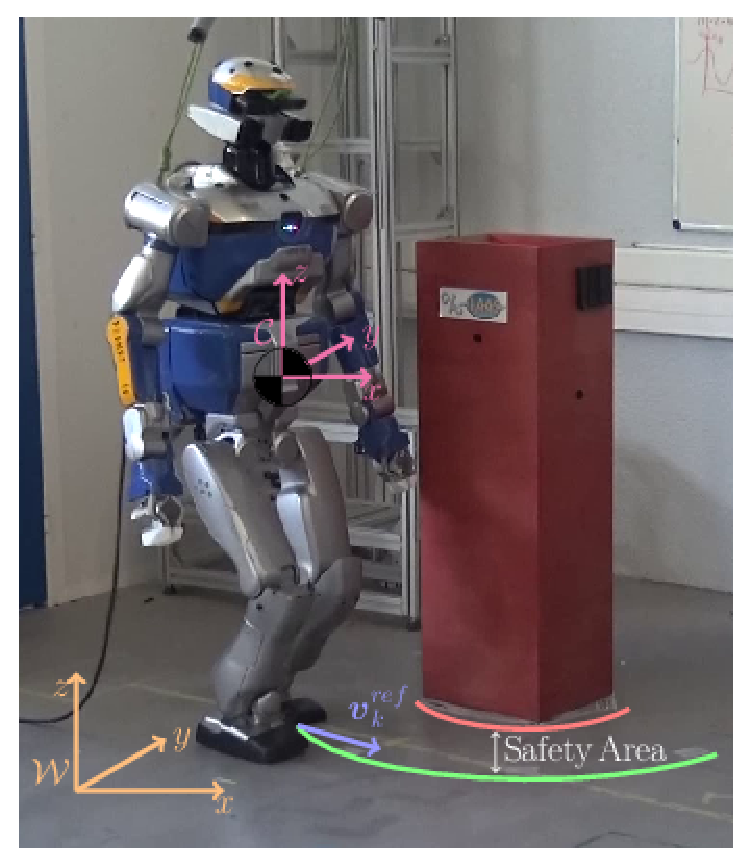
\includegraphics[width=0.7\linewidth, keepaspectratio]{./figures/synthesis}
%  \caption{HRP-2 is following an ellipse according the one-third power law. The center of gravity $\mathcal C$ is expressed in a global reference frame $\mathcal W$}
  \begin{tikzpicture}%[show background grid]% every node/.style={draw,outer sep=0pt,thick}]

% SoT
\draw [fill=green,opacity=.2,text opacity=1] (-1.5,2.2) rectangle (13.0,-2.2);
\node at(6,-2.0) {\textcolor{green!20!black!100}{Stack of Tasks}};

% Ellispe Reference
\node[rectangle,minimum width=2cm, minimum height=1cm,draw=blue!70,fill=blue!20] (ellipseref) at (4.0,3.25) {};
\node[ellipse,draw=blue,thick,minimum width=1cm,minimum height=0.5cm] at (ellipseref) {};
\node at ([yshift=-0.8cm]ellipseref) {Reference trajectory};

% Vector Field
\node[rectangle,minimum width=2cm, text width=2cm,minimum height=1cm,draw=blue!70,fill=blue!20,align=center] (vectorfields) at (0.0,0.0) 
{Vector Field\\
\includegraphics[scale=0.1]{two_third/Fig3e_EllipseBetaThird.pdf}
};
%\node at (0.0,2.5) {$\gamma,\beta$};

% Walking Pattern Generator
\node[rectangle,minimum width=2cm, minimum height=1cm,draw=blue!70,fill=blue!20]  (wpg) at (5.4,1.0) {Walking Pattern Generator};

% Task
\node[rectangle,minimum width=2cm, text width=3cm, align=center, minimum height=1cm,draw=blue!70,fill=blue!20] (ttt) at (11,1.0) 
{  Tasks for\\
   Trajectory\\
   Tracking};

% Solver
\node[rectangle,minimum width=2cm, text width=3cm, align=center, minimum height=1cm,draw=blue!70,fill=blue!20] (qp) at (11,-1.0) 
{ HQP Solver };

% Power Law
\node[rectangle,text width=2cm,align=center,minimum width=2cm, minimum height=1cm,draw=blue!70,fill=blue!20] (powerlaw) at (3.0,-1.0) {Power Law\\$\gamma,\beta$};
\path[->,>=stealth',draw=black] (vectorfields.314)-- node[below] {$\kappa$} (powerlaw.189);
\path[->,>=stealth',draw=black] (powerlaw.170)-- node[above] {$v$} (vectorfields.325);

% Robot
\node[rectangle,minimum width=2cm, minimum height=1cm,draw=blue!70,fill=blue!20] (robot) at (11,-3.5) {Robot};

% Localization
\node[rectangle,minimum width=2cm, minimum height=1cm,draw=blue!70,fill=blue!20] (localization) at (0.0,-3.5) {Localization};

%\path[->,>=stealth',draw=black] (0.0,2.25)-- (vectorfields.90);

% Links
\draw[->,>=stealth',draw=black] (ellipseref.180) -| (vectorfields.90);
\draw[->,>=stealth',draw=black] (vectorfields.42) -- node[above] {${\bf c}^*$} (wpg.180);
\path[->,>=stealth',draw=black] (wpg)-- node[above] {
$\begin{matrix}
{c}_{ref}\\{\bf z}_{ref}\\{\bf LF}_{ref}\\{\bf RF}_{ref}
\end{matrix} $
}(ttt);
\path[->,>=stealth',draw=black] (ttt)-- node[right] {\small Tasks} (qp);
\path[->,>=stealth',draw=black] (qp)-- node[xshift=0.2cm,yshift=-0.2cm,] {${\bf q}$} (robot);
\path[->,>=stealth',draw=black] (robot)-- node[below,font=\small] {Motion capture}(localization);
\path[->,>=stealth',draw=black] (localization)-- node[left] {${\bf w}$}(vectorfields);

\end{tikzpicture}

  \caption[Control scheme using the one third power law on HRP-2]{Power law based closed-loop control. An ellipse reference trajectory is specified and used, together with the power law defined by the velocity gain factor $\gamma$ and $\beta$ exponent constants, to generate the reference vector field. $(x,y,\theta)$ define the position and orientation of a frame attached to the robot's center of mass. The reference vector field defines center of mass velocity ${\bf c}^*=[\dot{x},\dot{y},\dot{\theta}]$ for the walking pattern generator. This particular walking pattern generator provides reference trajectories for the balanced center of mass ${\bf c}_{ref}$, the associated center of pressure ${\bf z}_{ref}$, and the feet ${\bf LF}_{ref},{\bf RF}_{ref}$. A whole body motion generator uses the reference trajectories to generate a command ${\bf q}$ realized by the robot (for HRP-2, this is the configuration vector). The localization component uses position measurements to provide a position ${\bf w} \in SE(3)$ of the robot, that again is used as input to the vector field to provide the correcting velocity vector ${\bf c}^*$. This chapter shows that the closed-loop approach reduces motion drifts, but not entirely, and suggests that using human-like power laws may help robots to perform faster, more accurate, and more stable motion. 
}
  \label{fig:covertwothirdpowerlaw}
\end{figure}

\subsection{Power laws governing human motion}
The speed of human motion is characterized by the one-third power law behavior;
movement speed $v$ decreases when curvature $\kappa$ increases,
following the quantitative relation $\vv = \gamma \kappa^{-\beta}$,
with $\gamma$ the piecewise constant velocity gain factor and $\beta=1/3$ the exponent.
This law, often termed the two-thirds power law due to equivalent formulation determining
angular speed $A = \gamma \kappa^{2/3}$, was first found for drawing hand motion \cite{lacquaniti_law_1983}.

Power law behaviors appear to emerge from jerk minimization \cite{huh_spectrum_2015}. Alternatively, the specific one-third power law, which is equivalent to moving with a constant equi-affine speed \cite{FlashHandzel1996}, may result from equi-affine metrics used by the human brain \cite{flash_affine_2007}, possibly in a mixture with Euclidean and full affine metrics \cite{bennequin_movement_2009}. 

Tuned to perception of biological motion, the human visual system perceives one-third power law motion as uniform, rather than movement with constant speed \cite{viviani_biological_1992}. Coupling between the motor and visual systems in the human brain is supported by stronger and more widespread brain activation patterns \cite{dayan_neural_2007}, and greater event-related desynchronization \cite{meirovitch_alpha_2015}, occurring when subjects watch one-third power law motion, compared with other power law motions.  Even imagined movements slow down in curved regions according to the one-third power law \cite{papaxanthis_relation_2012,karklinsky_timing_2015}. 
These evidences suggest that humans will perceive a humanoid robot moving according to the one-third power law as more human-like, finding his motions more predictable and easier to follow.

\subsection{Guiding trajectories for humanoid robots}
Planning humanoid robot locomotion is classically accomplished by constructing an optimal sequence of footstep transitions,
taken from a discrete set of possibilities,
that is kept small to allow reasonable computation time \cite{Chestnutt:2010:MPHR,Hornung:ICHR:12}.
The limitations of this approach in restricted scenarios yield an alternative approach; planning a reference trajectory which allows generation of the needed contacts \cite{perrin:iros:2011}.
This reference trajectory is usually generated considering balance constraints and geometrical constraints such as feasibility and manipulability. 
This approach significantly reduces the burden on the motion planner, but raises the demand for controllers capable of finding footsteps or contacts in real time.
Planning general contacts is still a very hard problem \cite{Escande:RAS:2013}, and finding a center of mass trajectory for a given set of contacts was only recently accomplished \cite{carpentier:hal-01203507}. For the restricted case of walking on flat ground, several new approaches \cite{deits:ichr:14,naveau:ral:2016,herdt:iros:2010} allow automatic finding of footstep positions. Therefore, it is now possible to move a humanoid robot by providing only a reference trajectory \cite{naveau:ral:2016, herdt:iros:2010}.

In the current study, we attempt to robustly regulate the walking motion on flat floor given a planned reference trajectory. A stable regulation process is important for correcting drifts, that appear due to the interaction of the humanoid robot's soles with the ground \cite{stasse:iros:2006}. The closed-loop control does reduce the drift. However, in this study we observe that the speed profile of the reference trajectory is crucial. The naive approach of close-loop regulation to obtain constant reference speed is unsatisfactory for HRP-2; a steady-state error is still apparent. Speed modulation according to the one-third power law nullifies this drift entirely.



\subsection{Robust trajectories with contracting dynamics}
Contracting dynamics provide a robust control policy for generating motion patterns; in presence of bounded noise exponential time convergence to a limit cycle or point is guaranteed \cite{lohmiller_contraction_1998}. By mapping an attractor of a contracting dynamical system to a movement primitive, Giese et al.~\cite{giese_realtime_2009} suggested a general control method for high dimensional systems. In robotics, contraction was already used for robust synchronization of phases of control pattern generators \cite{seo_cpg_2010} as well as for learning a set of dynamic motion primitives \cite{Perk2006}. 
In this work, we show how contracting dynamics are useful to robustly generate kinematic power law behavior. 

% ADDED BY MATAN:	
\section{Reactive walking pattern generator}

\input{WalkingPatternGenerator}

\section{Regularization of contracting oscillators}
\label{sec:regularization_contracting_oscillators}

In this section we will use the work done by M. Karklinsky and A. Mukovskiy and presented in \cite{matan:biorob:2016}.
For a given reference trajectory M. Karklinsky and A. Mukovskiy designed a contracting system using Andronov-Hopf oscillator.
The reference trajectory is a specific solution of the global dynamics. 
As a reminder, a dynamical system is contracting if all solutions in the contraction region converge exponentially to each other.
If a dynamical system is contracting, there exists an attractor in this contraction region, and all trajectories in the region converge exponentially to it \cite{lohmiller_contraction_1998}.
Contraction guarantees the exponential decays of
perturbations.
Partial contraction is contraction towards any of the particular solutions residing inside the flow-invariant manifold of the dynamics \cite{pham_stable_2007}.
For the current work, it suffices that the reference trajectory is an invariant one dimensional submanifold of partially contracting dynamics, with local contraction towards but not along the trajectory.
The partial contraction is easy to construct for an arbitrary trajectory, as demonstrated by M. Karklinsky and A. Mukovskiy in \cite{matan:biorob:2016} for cyclic trajectories.
Trajectories that are the natural test ground of power laws in human motion.
Each partially contracting system are regularized to obey a power law on all orbits, including the reference trajectory. 

\subsection{Morphed Andronov-Hopf oscillators}
This section recalls the construction of a stable dynamical system with desired limit cycle trajectory from an angular morphing of the basic Andronov-Hopf oscillator.

\subsubsection*{Angular morphed Andronov-Hopf oscillator}

The Andronov-Hopf oscillator \cite{park2009design}:
\begin{eqnarray}
\label{eq:angulardynamics}
\dot{\theta} &=& \omega\\ \nonumber
\dot{\rho} &=& \alpha(1-\rho)
\end{eqnarray}
With the winding angle $\theta$ and radius $r_0(\theta)$, defined as the orientation of the path's normal and its radius of curvature.
They are the direction and radius of the osculating circle as well.
$\rho=\frac{1}{r^2}=\frac{1}{x^2+y^2}$, $x,y$ being the Cartesian coordinates.
And with $\omega,\alpha>0$ being two constants.
For a path with positive (negative) curvature everywhere, like elliptic curves, the direction and radius of the osculating circle define $(\theta,r_0(\theta))$ at each point.
These coordinates on the path naturally extend to coordinates that cover a band around it.
For a constant $B = \min_\theta(r_0(\theta))-\epsilon>0$, in the compact band of width $B$ around the path, each point in the $(x,y)$ plane will map locally to one closest point with coordinates $(\theta,r_0)$.
Its coordinates will therefore be $(\theta,r(\theta))$; the winding angle and the distance from the center of the osculating circle of the closest point. 
To define a dynamical system on the angular coordinates, we define the coordinate $\rho(\theta) = \frac{1}{r^2(\theta)}=$, and use the dynamics from Eq.~\ref{eq:angulardynamics}.
It is partially contracting, since the Jacobian of the $\rho$ subsystem is uniformly negative definite $J_\rho<-\alpha<0$. 
This oscillator can be morphed \cite{ajallooeian_general_2013}:
\begin{eqnarray}
\label{eq:polarmorphingdynamics}
\dot{\theta} &=& \omega\\ \nonumber
\dot{\rho} &=& \alpha (F(\theta)-\rho) + \omega \frac{d F}{d \theta}
\end{eqnarray}
It is still partially contracting, with $F(\theta) = \frac{1}{r_0^2(\theta)} = \kap^2(\theta)$ the squared path curvature.
Global partial contraction in the $\theta,\rho$ coordinates to the limit cycle results in partial contraction to the reference path in the band of width $B$.

%%%%%%%%%%%%%%%%%%%%%%%%%%%%%%%%%%%%%%%%%%%%%%%%%%%%%%%%%%%%%%%%%%%%%%%%%%%%%%%%

\subsection{Temporal regularization of a dynamical system}

In this section, we define the power law regularization of dynamical systems and examine the conditions for its applicability. Under reasonable conditions, the regularized dynamical system has exponential convergence to the limit cycle of the original system. For some special cases the regularized system is contracting.

\subsubsection{Power law regularization}
We focus on regularization with a power law $\vv = \HH(\kap) = \gamma \kap^{-\beta}$, with $\gamma$ a global constant and $\beta$ the exponent value. This is the basic most useful example of the general Euclidean invariant dependency of speed upon path geometry, $\vv = \HH(\kap,\kaps,\dots,\kapn)$ (see \cite{bennequin_movement_2009}).

\begin{mydef} 
	For a dynamical system $\dot{\xnv} = F(\xnv)$, and a power law $\vv = \HH(\kap)$, we define the $\HH$-regularization of $F$, denoted by $\dot{\xnv} = F_\HH(\xnv)$, as $F_\HH(\xnv) = \frac{F(\xnv)}{|F(\xnv)|} \HH(\kap(\xnv))$, with $\kap$ the curvature of the orbit at point $\xnv$.
\end{mydef}
At each point, the orbit of $F_\HH$ geometrically coincides with the orbit of $F$. Additionally, the speed along each orbit of $F_\HH$ satisfies the law $\HH$.
Each velocity vector has the same direction in both system $F_\HH$ and $F$, but but not necessarily the same norm.
Our power laws are positively monotone so the directions of flows of $F$ and $F_\HH$ match. 

\begin{myass} We consider a region $U$ which is a compact trapping region in the plane for $F$ without fixed points. We require that for $F$'s orbits $\kap$ is defined and bounded, and therefore $\HH$ is defined and bounded; for each $\xnv \in U$, $\HH(\xnv)\geq C_1>0$ for some global constant $C_1$. We require that $F$ has bounded speed $|F(\xnv)|<C_2$ for some global constant $C_2$.
\end{myass}

These assumptions guarantee that, if $F$ is contracting in $U$ to some limit cycle, then each solution converges globally exponentially to this limit cycle in $U$ (see Lohmiller and Slotine's \cite{lohmiller_contraction_1998}, Theorem 1). While we do not claim that $F_\HH$ is generally contracting, our assumptions yield global exponential convergence of $F_\HH$ to the limit cycle of $F$. This is true because  $|F_\HH(\xnv)| = \frac{\HH(\xnv)}{|F(\xnv)|} |F(\xnv)| \geq \frac{C_1}{C_2}  |F(\xnv)|$. The limit cycle of $F_\HH$ is geometrically identical to that of $F$, and movement on it obeys the $\HH$ power law.






\subsubsection{Curvature of the orbits of the circular Andronov-Hopf oscillator}
Power law regularization has singularities in inflection points and along straight trajectories; if $\kap=0$ and $\beta>0$, the power law speed is infinite. This can be overcome in several ways. For most practical needs the power law speed $\vv$ can be bounded; Viviani and Stucchi \cite{viviani_biological_1992} defined $\vv = \gamma (\kap+\alpha)^{-\beta}$, with some constant $\alpha>0$ preventing the singularity at $\kap=0$. Alternatively, we can restrict the discussion to regions of positive curvature. For the morphed Andronov-Hopf oscillators, around a planned cyclic trajectory with positive curvature, there exists a band of bounded nonzero curvature, guaranteeing that the regularization process will result in finite speeds. 

The dynamics of $\rho(\theta)$ define $\kappa(\rho)$ along each orbit. For circular Andronov-Hopf oscillators, the dynamics are invariant with respect to rotations around the origin $(x,y)=0$. Therefore local curvature of the vector flow $\kappa(\rho)$ is a function of $\rho$ only, independent of $\theta$. For any integral trajectory its local curvature $\kappa(\rho)$ equals zero exactly where it crosses a circle $\rho_{\kappa=0}$ concentric to the unit limit cycle and bigger. Therefore, in the circular band $C\geq\rho\geq \rho_{\kappa=0}+\epsilon$, for arbitrarily small $\epsilon$ and arbitrarily large $C$, the curvature is strictly positive $\kappa\geq C_1>0$, speed is bounded, and our assumptions hold, allowing power law regularization that results in exponential convergence to the limit cycle. 


\subsubsection{A contracting one-third power law regularized elliptic oscillator }
For the one-third power law, any elliptic system generated as a linear transformation of the regularized unit circle oscillator is contracting. The argument of the unit circle regularized oscillator, based on the circular symmetry of $\kap$, holds for uniform scaling. A global equi-affine transformation of the plane conserves the one-third power law and therefore the transformation of the unit circle dynamics to elliptic dynamics using the combination of a scaling and an equi-affine transformation conserves contraction of the regularized system.
As a consequence a velocity vector field can be computed from any elliptic reference trajectory.
This velocity vector field has the property to make a point mass converge toward the reference trajectory if this point mass track the velocity of this vector field.
In Fig.~\ref{fig:ellipsis:power:laws} we can see the initial unit cycle oscillator in subFig.~\ref{fig:ellipsis:power:laws}.a.
This unit cycle can be morphed without loss of the contracting property of the reference trajectory (see subFig.~\ref{fig:ellipsis:power:laws}.b).
The subFig.~\ref{fig:ellipsis:power:laws}.c-\ref{fig:ellipsis:power:laws}.f correspond to the velocity vector field regularized by the power law with $\beta = -1/3,0,1/3,2/3$.
We can easily see here the influence of $\beta$ on the vector field.
If $\beta$ is small the velocity will be high when the curvature is high.

\begin{figure}[ht]
	\centering
        \includegraphics[trim=0.3cm 0.3cm 0.3cm 0.2cm,width=0.5\linewidth]{./figures/morphing.pdf}
	\caption{Morphing and regularization of an Andronov-Hopf oscillator. a)~The unit cycle oscillator. b)~an elliptic morphing. c)-f)~Four power law regularizations according to $\beta = -1/3,0,1/3,2/3$ power laws respectively. Each regularization keeps directions but changes speeds of the elliptic vector field.}
	\label{fig:ellipsis:power:laws}
\end{figure}


%%%%%%%%%%%%%%%%%%%%%%%%%%%%%%%%%%%%%%%%%%%%%%%%%%%%%%%%%%%%%%%%%%%%%%%%%%%%%%%%
\section{Results}
In order to evaluate the effect of applying the one-third power law to humanoid robot walking, we integrated the two third power law inside the Stack-of-Task framework. We present dynamic simulations and real robot experiments testing motions generated by the walking pattern generator (Fig.~\ref{fig:covertwothirdpowerlaw}). We compared four different power laws (Fig.~\ref{fig:ellipsis:power:laws}), with exponents $\beta=-1/3,0,1/3,2/3$. We explain the methodology and describe the results.

\begin{figure}[ht]
	\begin{center}
	  \includegraphics[height=0.25\linewidth]{./figures/RobotWalking.pdf} \hfill
	  \includegraphics[trim=2cm 9cm 0cm 12cm,clip=true,height=0.25\linewidth] 
	    {./figures/Fig5d_EXPshapesSymmetric.pdf}
  \end{center}
	\caption{Experimental setup, the robot walks according to a reference ellipse, obeying one of four different power law speeds. Trajectories for each power law converge around a limit cycle ellipse. }
	\label{fig:5def}
\end{figure}

% NEW ANALYSIS,Simulation:
% Symmetric algorithm
%Beta: -0.33 |D: 27.22 |A: 1.8196 
%Beta: 0.00 |D: 8.96 |A: 1.6615 
%Beta: 0.33 |D: 0.05 |A: 1.5726 
%Beta: 0.67 |D: 0.13 |A: 1.5695 

% Durations:
% 140.0025
% 134.0025
% 130.0000
% 127.2000
% % Power law betas for both, using curvature of shape:
%DS:Beta O: -0.33 |LL: -0.21 |U: -0.21 
%EXP: Beta O: -0.33 |LL: -0.22 |U: -0.23 
%DS:Beta O: 0.00 |LL: 0.05 |U: 0.05 
%EXP: Beta O: 0.00 |LL: 0.02 |U: 0.02 
%DS:Beta O: 0.33 |LL: 0.33 |U: 0.33 
%EXP: Beta O: 0.33 |LL: 0.36 |U: 0.34 
%DS:Beta O: 0.67 |LL: 0.62 |U: 0.60 
%EXP: Beta O: 0.67 |LL: 0.63 |U: 0.57 
%% R squared (simulation, experiment)
%0.4599    0.7011
%0.2741    0.0318
%0.9905    0.7933
%0.9441    0.8953

%% With experiment sway removal - BAD FOR SPEEDS!
%DS:Beta O: -0.33 |LL: -0.21 |U: -0.21 
%EXP: Beta O: -0.33 |LL: -0.21 |U: -0.31 
%DS:Beta O: 0.00 |LL: 0.05 |U: 0.05 
%EXP: Beta O: 0.00 |LL: -0.05 |U: -0.12 
%DS:Beta O: 0.33 |LL: 0.33 |U: 0.33 
%EXP: Beta O: 0.33 |LL: 0.35 |U: 0.32 
%DS:Beta O: 0.67 |LL: 0.62 |U: 0.60 
%EXP: Beta O: 0.67 |LL: 0.68 |U: 0.67 
% r s
%0.4565    0.1097
%0.2720    0.0217
%0.9904    0.0994
%0.9443    0.2941
\begin{table}[h]	
	\centering % centering table
	\begin{tabular}{||c||cc|c|c|c||} % creating 5 columns
		\hline
		\hline
		SIM    &  &    & & &\\
		Ref.~$\beta$     & Sim.~$\beta$ & $R^2$   & MSD (cm$^2$)& A (m$^2$)&T (s)\\
		\hline
		$-0.33$ & $-0.21$ & $0.46$ & $27.22$  & $1.820$ & $140.0$ \\
		$0$     & $ 0.05$ & $0.27$ & $8.96$   & $1.661$ & $134.0$ \\ 
		\textcolor{red}{$0.33$}  & \textcolor{red}{$0.33$}  & \textcolor{red}{$0.99$} & \textcolor{red}{$0.05$}   & \textcolor{red}{$1.573$} & \textcolor{red}{$130.0$} \\
		$0.67$  & $0.60$  & $0.94$ & $0.13$   & $1.569$ & $127.2$ \\
		\hline
		\hline
		EXP     &  &    & & &\\		
		Ref.~$\beta$     & Exp.~$\beta$ & $R^2$   & MSD (cm$^2$)& A (m$^2$)&T (s)\\
		\hline
		$-0.33$ & $-0.23$ & $0.70$ & $53.13 $ & $1.888$ & $150.4$ \\
		$0$     & $ 0.02$ & $0.03$ & $30.51 $ & $1.812$ & $142.4$ \\
		\textcolor{red}{$0.33$}  & \textcolor{red}{$ 0.34$} & \textcolor{red}{$0.79$} & \textcolor{red}{$39.00$} & \textcolor{red}{$1.855$} & \textcolor{red}{$134.4$} \\
		$0.67$  & $ 0.57$ & $0.90$ & $46.11 $ & $1.884$ & $133.6$ \\
		\hline
		\hline
		REF    & $-$     &$-$     & $0$      & $1.571$ & $120.0$ \\
		\hline
		\hline
	\end{tabular}	
	\caption{Results from dynamic simulation (SIM) and actual robot experiment (EXP); for different reference power laws (Ref.~$\beta$), simulated power law exponent (Sim.~$\beta$) and actual motion power law exponent (Exp.~$\beta$) calculated using nonlinear regression \cite{maoz_noise_2005} with R squared error ($R^2$), mean squared distance to the reference path (MSD), area (A) and duration (T) of the generated ellipse trajectory are given, with those of the reference frame (REF). Geometrically, in simulation the one-third power law, $\beta=1/3$, is most exact, and in experiment the constant speed was more exact. Temporally, higher $\beta$ exponents yield faster  motions for both simulation and experiment, but always slower than the reference.}
	\label{table:dynamicsimulationsummary}
\end{table}
 % Experiment, cleaned with new
%Beta: -0.33 |D: 53.13 |A: 1.2020 | 
%Beta: 0.00 |D: 30.51 |A: 1.1538 | 
%Beta: 0.33 |D: 39.00 |A: 1.1812 | 
%Beta: 0.67 |D: 46.11 |A: 1.1999 | 
%1.8881
%1.8124
%1.8554
%1.8847


% EXPERIMENT, with one lap same as before
%MSD
%54.6913
%31.3508
%40.0416
%46.9112
%AREA
%1.8931
%1.8165
%1.8602
%1.8882

% Duration
% 150.3750
% 142.3925
% 134.3975
% 133.6125

% area (aaa)
%1.9454
%2.0069
%1.9272  * smallest!
%2.0018

% actual results for table
%msd (ddd)
%79.7895
%114.1826
%69.9704    * smallest
%87.6226

%%%%%%%%%%%%%%%%%%%%%%%%%%%%%%%%%%%%%%%%%%%%%%%%%%%%%%%%%%%%%%%%%%%%%%%%%%%%%%%%%%%%%%%%%%%%%
%%%%%%%%%%%%%%%%%%%%%%%%%%%%%%%%%%%%%%%%%%%%%%%%%%%%%%%%%%%%%%%%%%%%%%%%%%%%%%%%%%%%%%%%%%%%%
\subsection{Integration inside the Stack-of-Tasks framework}

Fig.~\ref{fig:covertwothirdpowerlaw} present the architecture of the system.
It shows that the "Vector Field" output is $\bf c^*$, but in fact the vector field only provides linear velocity assuming that the robot is heading forward.
Hence, inside the vector field box there is a Proportional Integrative Derivative (PID) controller which track the orientation of the velocity vector.
It tries to minimize the error $e=atan(\frac{\dot{y}}{\dot{x}}) - \theta$.
With $[\dot{x} \; \dot{y}]$ the linear velocity extracted from the vector field and $\theta$ the orientation of the robot base.
The singularities of the $atan$ function is dealt with inside the PID controller.

The control period of the HRP-2 robot is $5\,ms$.
$2\,ms$ are consumed by the walking pattern generator, $1\,ms$ by the QP solver and $1\,ms$ by the robot low level controller which includes the stabilizer.
The vector field has $1\,ms$ left to be computed.
Hence, in terms of computation time, we had to include efficient C++ code inside the Stack-of-Tasks.

\subsection{Dynamic simulation results}

\begin{figure}
	\centering
	\includegraphics[trim=0cm 0.4cm 0cm 0.5cm,width=\linewidth]{./figures/dynamic_simulation.pdf}
	\caption{a)~Dynamic simulation paths, with different reference speeds. b)~Zoom in on the box in plot a. Simulations with positive $\beta = 1/3,2/3$ have no drift, less than $1$ cm from the reference path. Simulations with constant speed and negative power law $\beta = 0, -1/3$ drift outside of the reference elliptic path.}
	\label{fig:5ab}
\end{figure}


\subsubsection{Simulation and trajectory analysis}

To simulate motion, we used the OpenHRP simulator, that computes the contact forces and HRP-2's rigid body mechanics, and includes a model of the compliance of the robot ankles. We implemented the control architecture depicted in Fig.~\ref{fig:covertwothirdpowerlaw} in OpenHRP.
We analyzed the trajectories of the center of mass using MATLAB. To overcome the coronal swing motion we applied a procedure for finding the middle points of each sway. Each middle point was the average of two consecutive local signed curvature extrema with opposite signs, with time defined as the average of the times of these two points. We used the middle points trajectory for all analysis purposes. The values of the power law exponents $\beta$ were calculated using nonlinear regression estimation  \cite{maoz_noise_2005}. Repeating the procedure with $\log-\log$ linear regression yielded similar $\beta$ values. Speed was extracted from the middle points trajectory using a noise-insensitive filter \cite{Holobororodko2008}. Curvature was extracted from the reference ellipse.

\subsubsection{Power law patterns are reproduced}

The theoretical speed profiles are compared with the one measured in simulation (Fig.~\ref{fig:5g}, left) and the one measured from the motion capture system (Fig.~\ref{fig:5g}, right).
The simulation yielded positions of maximal speed slightly shifted with respect to maximal speed positions predicted by the power law based on the curvature of the actual path; for $\beta=-1/3,1/3,2/3$ shifts along the trajectory, of $22,4,-15$ cm of the simulated with respect to reference speed peaks occurred.
Unpredictably, constant speed $\beta=0$ power law yielded an oscillatory curvature-dependent speed profile. 
% OLD simulation:
% Beta: -0.33 |D: 0.22 
% Beta: 0.00 |D: 0.97 
% Beta: 0.33 |D: 0.04 
% Beta: 0.67 |D: -0.15 

\subsubsection{Drift correction by one-third power law}
As predicted, the simulated one-third power law resulted in reduced drift compared to constant speed and other power laws. For $\beta=1/3$ the path was most similar to the reference path, with next best being the $\beta=2/3$ power law. The constant speed $\beta=0$ and $\beta=-1/3$ yielded drifts; the simulated elliptic paths were larger than the reference elliptic path, as reflected by area and mean squared distance (see table \ref{table:dynamicsimulationsummary} and Fig.~\ref{fig:5ab}). Interestingly, the constant speed $\beta=0$ path deviated from the reference frame gradually and not immediately upon movement initiation, as seen in  Fig.~\ref{fig:5ab}.b.


\subsubsection{Increase in $\beta$ exponent decreases duration}
Simulated motions took more time than the reference time, that was always two minutes per lap. The power law exponent affected movement duration; the higher the $\beta$ the faster the motion, so its duration was closer to the reference behavior (table \ref{table:dynamicsimulationsummary}).


\begin{figure}[ht]
	\centering
	\includegraphics[trim=2cm 7cm 1cm 9.1cm, clip=true,keepaspectratio,width=0.8\linewidth]{./figures/Fig5g_DSspeedprofilesBoth.pdf}
	\caption{Speed profiles for dynamic simulations (Left) and robot experiment (Right), with four different reference speeds (Ref). Both simulated and actual robot motions reproduce the spatio-temporal power law patterns.}
	\label{fig:5g}
\end{figure}

% OLD: Simulation only
%\begin{figure}
%	\centering
%	\includegraphics[trim=2cm 7cm 2cm 9.1cm, clip=true,keepaspectratio,width=1\linewidth]{./figures/Fig5c_DSspeedprofilesSymmetric}
%	\caption{Dynamic simulation with different reference speeds (Ref). Only for $\beta=1/3$ the simulation matches reference speed. Constant reference speed simulation slows near planned curvature maxima (perpendicular gray lines). The locations of speed maxima of the simulated trajectory ($\blacklozenge$) and reference trajectory ($\bullet$) for $\beta=1/3$, differed by a $4$ cm distance, less than for $\beta=-1/3,\beta=2/3$, that had more than $15$ cm distances. We calculated reference speeds using curvature of the actual path.}
%	\label{fig:5c}
%\end{figure}


%%%%%%%%%%%%%%%%%%%%%%%%%%%%%%%%%%%%%%%%%%%%%%%%%%%%%%%%%%%%%%%%%%%%%%%%%%%%%%%%%%%%%%%%%%%%%
%%%%%%%%%%%%%%%%%%%%%%%%%%%%%%%%%%%%%%%%%%%%%%%%%%%%%%%%%%%%%%%%%%%%%%%%%%%%%%%%%%%%%%%%%%%%%

\subsection{Experimental results}
\subsubsection{Experimental setup and trajectory analysis}
We tested the four power laws with the actual HRP-2 robot; the robot started standing approximately $60$ cm behind the tip of the ellipse, and walked until completing two laps. We used center of mass trajectories measured with the motion capture system, low pass filtered at $0.1$ Hz.  Analysis was identical to that of simulated motion.  


\subsubsection{Power law patterns are reproduced}
The reference speed power laws were noisily reproduced by the robot (see table \ref{table:dynamicsimulationsummary} for $\beta$ values and their $R^2$ errors, and figure \ref{fig:5g} for speed profiles). 

\subsubsection{Geometrical drift does not fully vanish}
Overall, experimental results showed larger drifts than simulation. The constant reference speed resulted in the lowest drift (table \ref{table:dynamicsimulationsummary}), outperforming the positive $\beta$ power laws. Different convergence trajectories (see figure \ref{fig:5def}), may arise from different initial positioning. 
 
\subsubsection{Increased $\beta$ decreases duration}
The actual movement of the robot took longer time than simulation. The trend we reported for the simulations; the higher the $\beta$ the faster the motion, was fully reproduced in the experiment.

\subsubsection{Evaluating controller corrections}

\begin{table}[ht]
	\centering 
	\begin{tabular}{|| c || c | c | c | c ||c |} 
		\hline 
		\hline 
		Ref.~$\beta$        & $-0.33$  & $0$      & \textcolor{red}{$0.33$} & $0.67$   \\
		\hline  
		Norm     (m)        & $1.416$  & $0.950$  & \textcolor{red}{$0.642$} & $1.124$ \\   
		Orientation (deg)   & $76.83$  & $89.60$  & \textcolor{red}{$60.45$} & $77.28$ \\ 
		Force ($kN\times$s) & $21.93 $ & $23.54$  & \textcolor{red}{$19.80$} &$21.01$  \\ 
		\hline
		\hline 		  
	\end{tabular}
	\caption{Analysis of the odometry frame and forces. For each of the four power laws the distance from center (Norm), body orientation (Orientation) and integrated norm tangential force measured on ankle (Force) are given. The one-third power law is outperforming all other power laws.}
	\label{tab:odometry_drift}
	
\end{table}

To estimate the  feedback correction done by the vector field and the PID controllers, we analyzed the internal odometry frame of the walking pattern generator. For each reference power law we examine the last crossing point of center of mass trajectory with the $x$ axis. We measured deviation from the baseline, the planned position and orientation, to gain error values reflecting the accumulated error along the two laps, caused by sliding . Additionally we examined tangential forces on the ankle, indicating the amount of compensated sliding. The one-third power law showed smaller accumulated errors, compared to the other power laws (table \ref{tab:odometry_drift}). Less error needing compensation implicates lower burden on the hardware.
 
%\begin{table}[h]
%  \centering 
%  \begin{tabular}{|| c || c | c | c | c |} \hline 
%    $\beta$     & -1/3    & 0.0    & 1/3    & 2/3    \\ \hline  
%    Norm        & 1.416   & 0.950  & 0.642  & 1.124  \\ \hline  
%    Orientation & 76.83   & 89.598 & 60.453 & 77.217 \\ \hline 
%  \end{tabular}
%  \label{tab:odometry_drift}
%\end{table}


\section{Conclusions}

In simulation and experiment, we tested how stable generation of power laws may help humanoid robot walking. 
The simulations and experiments reproduced the reference power law's temporal patterns.
The one-third power law, used by humans, appears beneficial for drift reduction. The one-third power law reduced drift in simulations and also resulted in less need for sliding compensation in actual robot motion.
Finally, our simulations and experiments showed that using higher $\beta$ exponent power laws allows faster movements. 

Having shown the importance of using a path-adjusted speed profile, it is still not fully determined how to select an optimal speed profile for stabilized and accurate robotic locomotion, given a planned reference trajectory. The different perspectives describing how the human motor system selects movement speed, based on either optimization \cite{flash_coordination_1985,todorov_optimal_2002} or geometric invariance \cite{flash_affine_2007,bennequin_movement_2009}, may prove beneficial for this aim. 

%To fully clarify the contribution of specific temporal patterns to different facets of human and humanoid locomotion is left for future studies.

%\subsection{From center of mass regulation to full body locomotion}
%Extending the regularities of a specific trajectory and forming globally converging dynamics is required to stably generate humanoid motion. Section \ref{sec:regularization_contracting_oscillators} addressed two issues. First, building a regulator around a given reference trajectory, is needed for spatial drift compensation during trajectory execution. Second, power law regularization allows transforming the temporal structure of a trajectory to a pace regulator on the plane. A systematic examination of these two processes is called for. Interestingly, defining the center of mass behavior is just the beginning. One example has to do with the necessity of contact switching from one footstep to another. In the current study, the time between footsteps was fixed and speed was realized by modifying the step length. However, freely determining contact times may improve the quality of the trajectory tracking.  
Except for systematic examination in locomotion of the benefits of different speed regularities, we suggest two additional applications of the speed modulation according to the geometry of the reference trajectory. One is to use power laws as a constraint for kino-dynamic motion planning  \cite{Pham:rss:2009}, the other is to find bounds on curvature when planning the motion of the free-flyer \cite{Orthey:PhD:2015}. 

%The pattern generator used in this system is the predominant source of constraints which do not allow perfect tracking of the guiding trajectory. 


%In this study, all the constraints are either purely mechanical or motivated by the
%control one-third power law, as they are the constraints formulated in the optimization problem solved for walking.
%The evident benefit for humanoid motion of the one-third power law may be based upon deep characteristic properties that are common to the two legged motion of both humans and humanoids. Finding these properties is left for future work.


%\subsection{}
%[] Containing: Problems, analyze them, extensions]
%\begin{itemize}
%	\item Why is 2/3 power law better?
%	\item Problem of 
%
%\end{itemize}

%\subsection{Dynamical systems for generation of robust cyclic behavior}
%
%\subsection{Temporal and geometrical aspects of the }
%\subsection{Regularization of dynamical systems}
%[XXX put here or in the methods?]
%The process of power law regularization, which we applied on the morphed Andronov-Hopf oscillators, is a specific instance of a more general process of speed regularization. For an arbitrary dynamical system and an arbitrary regularity law of motion, determining how speed is dependent on geometry of trajectories, the regularization process is applicable wherever $H$ is well defined. Wherever the original dynamics converge and the regularity law is monotone (a curve parametrization with no zero speed), the regularized dynamics are also converging. If the original dynamics are exponentially converging and the change of speed induced by the regularization is bounded then the regularized dynamics are also exponential. This happens if the original system is contracting, but also in other cases. A natural question is what conditions guarantee that a regularization law conserves contraction, namely transforms an original contracting system to a regularized contraction system. We have proven that the one-third power law regularization of an area-preserving morphing [XXX equi-affine?] of the basic Andronov-Hopf oscillator, this is the case. 
%
%[XXX Tamar: do you think we should omit this or keep?]
%Power laws in general, and specifically the one-third power law, can not describe movement through inflection points, as predicted speed goes to infinity. This drawback was resolved by the work of Bennequin et al. \cite{bennequin_movement_2009} which incorporated Euclidean, equi-affine and full-affine geometries in the mixed geometries model, to account for movement speeds along general trajectories. The regularization process proposed here is easily extendable to a mixed-geometry regularization process. 
%
%Another alternative description of movement speed along a desired trajectory is 
%  
%
%\subsection{Coordinate systems for convergence to a trajectory}
%
%\subsection{From center of mass trajectories to multiple dimensions}

%%%%%%%%%%%%%%%%%%%%%%%%%%%%%%%%%%%%%%%%%%%%%%%%%%%%%%%%%%%%%%%%%%%%%%%%%%%%%%%%
\chapter{Learning Movement Primitives for the Humanoid Robot HRP2}
\label{chap:primitives}

\ifdefined\included
\else
\minitoc
\minilof
\fi

\cleardoublepage

Skilled human behavior is highly predictive and relies on predictive planning.
It adapts its behaviors according to task constraints with relevance for
motor behaviors in the future.
Recent work in predictive control has shown great promises for generating complex behaviors \cite{Koenemann:iros:2015}.
They are however important combinatorial challenges.
In this chapter we propose a control framework combining biologically-inspired online planning for the robot upper body and model predictive control for the robot lower body.
The two controllers are linked together using a model predictive control method.
The computational foot print can be compared to the model predictive control presented in \cite{herdt:iros:2010}.
The human-like upper body motion is generated via a network of coupled dynamical movement primitives.
This network is embedded within a nonlinear dynamical system that generates coordinated behavior.
The lower body is controlled by the walking pattern generator presented in Chap.~\ref{chap:nmpc}.
This combination ensures the flexibility of the system as well as the safety of the robot.

This chapter is structured as follows: we will present the motivation behind this work in Sec.~\ref{intro}. A quick overview of related works in areas of computer graphics and humanoid robotics is given in Sec.~\ref{relatedworks}.
Then, in Sec.~\ref{sc:SystemArchitecture}
we will explain successively the top down approach, the bottom up approach and the overall architecture of the controller.
Finally, in Sec.~\ref{sc:Results} some preliminary results are presented, which demonstrate the feasibility of the approach in simulation and on the real HRP-2 robot.
This work is done in the frame of a collaboration with our colleague, experts in human motion analysis, in the \koroibot\ project.
This chapter is based on the submitted paper \cite{mukovskiy:jras:2016}.
The video of the application can be found at \url{https://youtu.be/3LT_QEiZzSo}.


\section{Motivation}
\label{intro}

The modeling and the synthesis of online-reactive multi-action sequences
are important topics both in computer graphics and in humanoid robotics.
The most challenging part of the online control of complex whole-body behaviors is the coordination of the different tasks.

In the current work we present a novel approach that combines the walking pattern generator (WPG) presented in Chap.~\ref{chap:nmpc},
with an online kinematic planning architecture for full-body movements.
The upper body motion pattern generator is based on learned dynamical movement primitives.
And the lower body motion generator is based on model predictive control.
The approach is suitable for the online planning and control of reactive behaviors that integrates locomotion and reaching.
It also includes highly flexible re-planning even in short time horizons.
The locomotion planned by the WPG is combined with the planned motion of the upper body using the dynamic filter presented in An.~\ref{an:dyn:filter}.
This ensures that the overall behavior results in a dynamically stable gait with the predefined CoM velocities and predefined upper body motion.
The proposed method is characterized by a much smaller computational complexity than a direct motion planning using complex dynamical model.
The global computational complexity can be compared with the one of standard WPG algorithms \cite{herdt:ar:2010}.

\section{Related work}
\label{relatedworks}

The general problem of motion generation in a dynamic environment is challenging.
The continuous change of the environment and error in state estimations implies a relatively high control frequency, typically at least 10 HZ.
It also implies a reasonable preview horizon duration, typically at least $2$ steps or around $1.6\,s$ for a human size robot.
Solving a model predictive control problem for a humanoid robot with $30$ degrees of freedom in a horizon of $1.6\,s$ is still an open issue.
This implies that a priori knowledge or approximation of the problem lowering the complexity is needed.

Current solutions range from near real-time whole body Model Predictive Control with
regularized modeling of contacts in order to decrease the associated computational cost
\cite{tassa:iros:2012,Koenemann:iros:2015}.
To a precise modeling of contact phases, which requires hours of offline computation time \cite{ref:km12}.

Another challenging issue for the generation of human-like behaviors is the sequential planning of
multi-step sequences, where individual steps can be associated with different
sub-goals or constraints (like contact with goal objects or step-length constraints).
This problem being multidisciplinary, we quickly review associated work in computer graphics, biological motor control, and humanoid robotics.

\subsection{Modeling of whole-body movements in computer graphics}
The problems of kinematic synthesis of such complex whole body movements has been addressed
extensively in computer graphics, e.g. \cite{ref:lwhpk12}, and many learning-based approaches
have been proposed that provide low-dimensional parametrization of classes of whole body motion \cite{ref:wfh08}. Recently, more attention has been given
to  methods for the blending of learned motion primitives, whose concatenations over time have to
satisfy  additional task constraints.  For example, in \cite{ref:fxs12} captured motion samples were
blended exploiting a prioritized 'stack of controllers'. In \cite{ref:smkb14} the
instantaneous blending weights of controllers were prioritized by their serial order.
In \cite{ref:hk14} the coordination between locomotion and arm pointing in the
last step was modeled by blending and selecting arm pointing primitives dependent
on the gait phase.

\subsection{Biological motor control of multi-step sequences}
Human motor behavior including action sequences has been shown to be highly predictive.
This has been investigated, for example, in a recent study on the coordination of walking
and reaching \cite{ref:lrss13}. Human subjects had to walk towards a drawer and to
grasp an object, which was located at different positions in the drawer. Participants
optimized their behavior already multiple steps before the object contact, consistent with the
hypothesis of \emph{maximum end-state comfort} during the reaching action \cite{ref:ws10, ref:r08}.
This means that the steps prior to the reaching were modulated in a way that optimizes the distance
for the reaching action \cite{ref:lrss13}. In  \cite{ref:mlsg15} our partners have proposed a
learning-based framework that is based on movement primitives that are learned from motion capture data,
and which reproduces these human planning strategies for an application in computer animation.
The underlying architecture is simple and approximates complex full-body movements by
dynamic movement primitives that are modeled by nonlinear dynamical systems. These primitives
are constructed from kinematic primitives that are learned from trajectory sets by anechoic demixing.
Similar to  related approaches in robotics \cite{ref:gam08,ref:buc06}, the method generates complex
movements by the combination of a small number of learned dynamical movement primitives. Our partners have previously
demonstrated the advantages of this approach for the adaptive online generation of multi-step sequences
with coordinated arm movements \cite{ref:mlsg15, ref:gie09}.

\subsection{Related approaches in humanoid robotics}
Several  approaches have  been proposed in robotics for the synthesis of
walking combined with grasping movements. Indeed, the DARPA robotic challenge
valve manipulation task forced the researchers to find efficient and robust methods
to perform reaching and manipulation tasks. \cite{ref:Ajoudani2013} proposed
a hybrid controller, where the robot is using a goal-driven fast foot step planner in combination
with visual servoing for the reaching and grasping of the valve.
\cite{ref:kuindersma2015optimization} proposes
a complete control architecture for the humanoid robot Atlas that is able to localize the robot
and automatically finds foot step around or over obstacles in order to reach a user defined goal.
The architecture contains also a whole-body controller which allow the robot to get
up from a lying down position, or to do complex task like turn the valve.
Another team (IHMC) presented an architecture in \cite{ref:johnson2015team} with a more sophisticated
control of the locomotion in \cite{ref:Englsberger2015}.
All three mentioned control architectures can make a humanoid robot reach, and then
grasp or manipulate objects as required for the robotic challenge.
To our knowledge an online simultaneous coordination of both tasks has not been demonstrated so far.
Other solutions for the combination of walking and vision-controlled reaching of a static and mobile target during walking were proposed in \cite{ref:svdmsvey08} and \cite{ref:bjkeht13}.

Randomized motion planning methods allow the generation of complex whole body motion  in constrained environment but at a high computational cost \cite{ref:dklntl13,ref:kly11}.
\cite{ref:gtg10}  proposed an algorithm for the computation
of optimal stance locations with respect to the position of a reaching target, where a dynamical systems
approach was used to generate the reaching behavior.
\cite{yoshida2007give} used a task priority approach,
based on a  generalized inverse kinematics, in order to organize several sub-tasks, including stepping, hand motion,
and gaze control.
Other work has exploited global path planning in combination with walking pattern generators (WPGs) \cite{Kajita:icra:2003} in order to generate collision-free dynamically stable gait paths.

A first attempt to transfer human reaching movements to humanoid robots by using motion-primitives was proposed in
\cite{ref:ttsg13}. In this work the primitives were extracted by using PCA and the behavior was successfully
implemented on the HRP-2 robot, only involving the trunk and arm joints.
The use of motion primitives in robotics
was also proposed in \cite{ref:gnzwiau13}, also including the integration of force-feedback.
\cite{ref:inhps13} and \cite{ajallooeian_general_2013} proposed systems based on dynamical movement primitives that
can be  modulated in real-time for the generation of complex movements.
However their approach focus on learning the in an efficient way the input data.
In \cite{ref:inhps13} the transfer to robot is tackled by using a low level torque controller managing the feasibility of the system.
This could result in a different motion than the one learned.
So the transfer from balanced human locomotion to balanced robot locomotion is still an open question.

\section{System architecture}
\label{sc:SystemArchitecture}

\begin{figure}[ht]
\centering
\renewcommand{\picturefontsize}{\LARGE}
\renewcommand{\pictureLineWidth}{0.8mm}

% For every picture that defines or uses external nodes, you'll have to
% apply the 'remember picture' style. To avoid some typing, we'll apply
% the style to all pictures.
\tikzstyle{every picture}+=[remember picture]
\tikzstyle{na} = [baseline=-.5ex]

\def\localarrow{
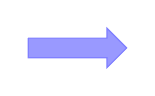
\begin{tikzpicture}
\path[draw=blue!50,fill=blue!40] (0,0.125) -- (1.0,0.125) -- (1.0,0.25) -- (1.25,0.0) -- (1.0,-0.25) -- (1.0,-0.125) -- (0.0,-0.125) -- (0.0,0.125);
\end{tikzpicture}
}

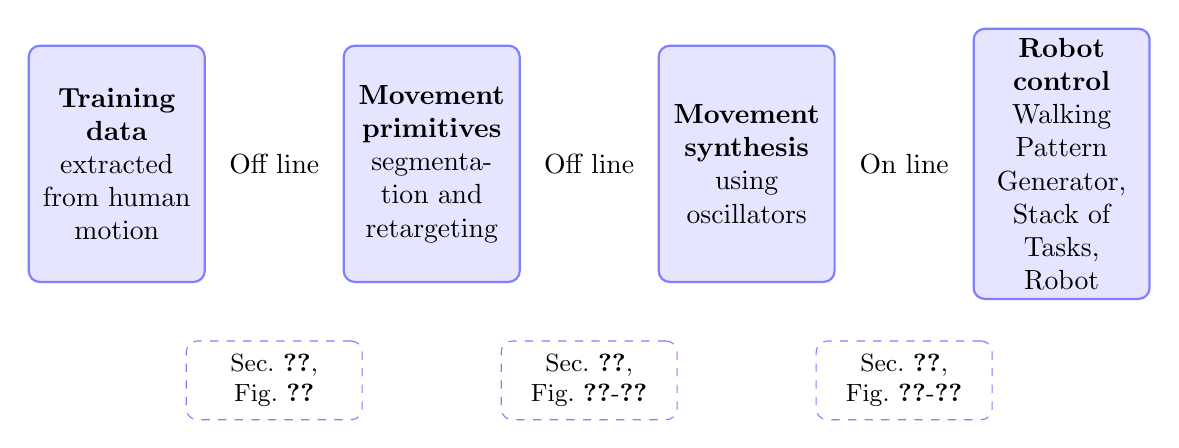
\begin{tikzpicture}%[show background grid]% every node/.style={draw,outer sep=0pt,thick}]

% Rectangle
\node (trainingdata) [text centered, shape=rectangle,rounded corners,draw=blue!50,fill=blue!10,thick,text width=2cm, minimum height=3cm]
  at (0.0,-0.5) {\textbf{Training data} extracted from human motion};

\node (movementprimitives) [text centered, shape=rectangle,rounded corners,draw=blue!50,fill=blue!10,thick,text width=2cm, minimum height=3cm]
  at (4.0,-0.5) {\textbf{Movement primitives} segmentation and retargeting};

\node (movementsynthesis) [text centered, shape=rectangle,rounded corners,draw=blue!50,fill=blue!10,thick,text width=2cm, minimum height=3cm]
  at (8.0,-0.5) {\textbf{Movement synthesis} using oscillators};

\node (robotcontrol) [text centered, shape=rectangle,rounded corners,draw=blue!50,fill=blue!10,thick,text width=2cm, minimum height=3cm]
  at (12.0,-0.5) {\textbf{Robot control}\\Walking Pattern Generator,\\ Stack of Tasks,\\ Robot};

\node (firstarrow) at (2.0,0.25) {\localarrow };

\node (trainingdatalabel) [text centered, shape=rectangle,rounded corners,draw=blue!50,fill=white,dashed,text width=2cm, minimum height=1cm,font=\small]
  at (2.0,-3.25)  {Sec.~\ref{subsec:modeling}, Fig.~\ref{fig:real}};

\node (sndarrow) at (6.0,0.25) {\localarrow };

\node (motionsynthesislabel) [text centered, shape=rectangle,rounded corners,draw=blue!50,fill=white,dashed,text width=2cm, minimum height=1cm,font=\small]
  at (6.0,-3.25) {Sec.~\ref{subsec:modeling}, Fig.~\ref{fig:Sources}-\ref{fig:RobotHuman}};

\node (thrdarrow) at (10.,0.25) {\localarrow };

\node (robotlabel)  [text centered, shape=rectangle,rounded corners,draw=blue!50,fill=white,dashed,text width=2cm, minimum height=1cm,font=\small]
  at (10.0,-3.25) {Sec.~\ref{sc:Implementation}, Fig.~\ref{fig:onlineWPG}-\ref{fig:zmpmb}};

\node[rotate=180] (rfirstarrow) at (2.0,-1.25) {\localarrow };
\node[rotate=180] (rsndarrow) at (6.0,-1.25) {\localarrow };
\node[rotate=180] (rthrdarrow) at (10.,-1.25) {\localarrow };

\node (offline1) at ( 2.0,-0.5) {Off line};
\node (offline2) at ( 6.0,-0.5) {Off line};
\node (offline1) at (10.0,-0.5) {On line};

\end{tikzpicture}

\caption{This graph represents a general overview of the system architecture}
\label{fig:archi:general}
\end{figure}

The global architecture of the system is depicted Fig.\ref{fig:archi:general}.
It is composed by two processes done offline.
The first is the data acquisition of human motion and the second is the segmentation and retargeting of this motion to be played on humanoid robots.
Then two blocks work in real time.
The first is the generation of the learned retargeted motion and the second is the controller of the humanoid robot.
More details are provided in the following section.

\subsection{Human data}
\label{subsec:modeling}

\subsubsection*{Drawer opening task}

The modeling of the coordination of walking and reaching was based on a motion
capture data set from humans who opened a drawer. The participants walked
towards a drawer, opened it with their left hand and reached for an object
inside with their right hand. The initial distance from the drawer and the position
of the object inside were varied \cite{ref:mlsg15}, see Fig.~\ref{fig:real}.
For more detail the reader is kindly asked to read \cite{mukovskiy:jras:2016}.
A video of the motion is available here \url{https://tinyurl.com/he3dhb2}.
The motion is cut into three different gait :
\begin{list}{ \arabic{point}.}{%
		\usecounter{point}%
		\setlength{\topsep}{5pt}%
		\setlength{\itemsep}{0pt}%
		\setlength{\parsep}{0pt}%
		\setlength{\labelwidth}{3.em}%
		\setlength{\leftmargin}{2em}%
		\setlength{\labelsep}{0.5em}%
	}
\item normal walking,
\item adaptive steps, i.e. walking motion plus reaching the drawer handle with the left hand,
\item grasping, i.e. stop walking plus reaching the target with the right hand.
\end{list}
\begin{figure}[ht]
  \centering
  \includegraphics[width=0.5\textwidth]{realavatar.jpg}
  \caption{Illustration of important intermediate postures of the human behavior:
    step with initiation of reaching, standing while opening of drawer, and reaching for the  object.}
\label{fig:real}
\end{figure}

\subsubsection*{Learning of the kinematic primitives}
\label{sc:Modeling}

In order to learn low-dimensional representation of every individual segmented motion we apply the anechoic demixing algorithm \cite{ref:og11, ref:caeg13}.
In this approach the joint angle trajectories are learned unsupervisely as an \emph{anechoic mixture model}: \newline
\begin{displaymath}
\underbrace{\xi_{i}(t)}_{angles}=m_i+\sum_{j}w_{ij}\underbrace{\sigma_{j}\left(t-\tau_{ij}\right)}_{sources}
\end{displaymath}
Here, for each angle trajectory $\xi_{i}(t)$ is represented as the linear mixture of $j$ source signals $\sigma_{j}(t)$ with the linear weights $w_{ij}$
plus the angle mean value $m_i$. 
These source signals can be delayed individually with time delays $\tau_{ij}$, which are different for different angles and source components.
Very good approximations can be computed with less than 4-5 learned source functions \cite{ref:gie09}.
In our standard implementation we first extract the mean angle values from our data.
Then we estimate the weights of additional non-periodic source component, which shape is usually given, but not inferred from the data. 
The shape function serving as nonperiodic source is taken as follows: $s_0(t)=cos(\pi t/T)$, where the time length of trajectory samples (and the period of periodic sources) is $T$.
For the first gait three periodic sources and a non periodic one were sufficient.
For the other two gait, the four sources did not provide a good enough approximation quality.
Therefore additional two sources were learned from the difference between the original trajectories and the learned one using three periodic sources and one non periodic.
Such constrained step-wise approach simplifies the blending between different motion styles, since then the delays of the sources are identical over styles.
The resulting shapes of learned source functions are presented in Fig.~\ref{fig:Sources}.

\begin{figure}[ht]
  \centering
  \includegraphics[width=0.48\textwidth]{sources4p2h.pdf}
  \caption{Extracted source signals.}
\label{fig:Sources}
\end{figure}

\subsubsection*{Online kinematic motion synthesis of multi-action sequences}

In order to make the rendering of whole-body trajectories online we propose an architecture built upon the
autonomous dynamical systems regarded as central pattern generators (CPGs), \cite{ref:gie09}. By this approach, our kinematic primitives
are generated online by dynamical systems, or dynamic primitives, DMPs \cite{ref:buc06, ref:inhps13}.
For this we map the solutions of the dynamic primitives onto source signals by Support Vector Regression (using a Radial
Basis Function kernel and the LIBSVM Matlab$^{\circledR}$ library \cite{ref:cha01}). The resulting architecture is summarized at
Fig.~\ref{fig:KinemPrimitivesArchitecture}.

\begin{figure}
  \centering
  \includegraphics[width=0.48\textwidth]{Graph_syst.pdf}
  \caption{Architecture for the online synthesis of body movements using dynamic primitives, \cite{ref:gie09}. This architecture is fused into one block named \textbf{Kinematic Pattern Synthesis} in Fig.~\ref{fig:onlineWPG} }
\label{fig:KinemPrimitivesArchitecture}
\end{figure}

For the periodic DMPs we chose a limit cycle oscillator (Andronov-Hopf oscillator) as canonical dynamics. It can be characterized by the differential equation system (with $\omega$ defining the eigenfrequency), for the pair of state variables $[x(t),y(t)]$:
\begin{eqnarray*}
\dot{x}(t) =[1-(x^2(t)+y^2(t))]x(t)-\omega y(t)\\
\dot{y}(t) =[1-(x^2(t)+y^2(t))]y(t)+\omega x(t))
\label{hopfosccoupl}
\end{eqnarray*}	
The online phase-shifting is modeled as an additional rotation of the oscillator phase plane, such that, due to the circular shape
of the attractor limit cycle of Andronov-Hopf oscillator, the trajectories on the attractor exhibit simple time-delays, c.f. \cite{ref:gie09}.
The instantaneous phase of the leading DMP also controls the start-triggering event for the non-periodic source. All the periodic DMPs
are phase-coupled in order to assure the coordinated globally stable dynamics. The methods of coupling was designed based on Contraction Theory, \cite{ref:par09}.

To model the actions with variable styles we do learning of nonlinear mappings between task parameters and action parameters (the sources weights).
This mapping is learned by Locally Weighted Linear Regression method (LWLR), \cite{ref:mlsg15}, and the relevant task parameters are steps lengths and timings.
For the synthesis of multi-step step sequences the step lengths are computed from the current estimated target distance. The simplified strategy taken for the
online synthesis is the following: the step lengths in the first action can be modified in range of training data (additional steps can be introduced by higher level
supervision algorithm, if target distance is too large); the step length in the second action is computed to realize maximum comfort distance for reaching. The smooth interpolation between the morphable weights of the kinematic primitives at the moments of concatenation of action is described with all technical details in \cite{ref:mlsg15}.

\subsubsection*{Processing}

\begin{figure}[ht]
  \centering
  \includegraphics[width=0.36\textwidth]{RobotAvatarjpg2.jpg}
  \caption{The result of the retargeting of the drawer opening task onto the unconstrained skeleton of the HRP-2 robot. The movie is available here [\url{http://tinyurl.com/j8qnbtp}}
\label{fig:RobotHuman}
\end{figure}

Once the recorded motion is learned, it is animated in MotionBuilder (Autodesk),
using an 'actor' puppet whose geometric parameters were adapted to the recorded subject.
The trajectory was first normalized in duration and mapped to the robot using the Denavit-Hartenberg (DH) convention.
The joint limits are not taken into account at this stage.
Fig.~\ref{fig:RobotHuman} is a frame of the movie [\url{http://tinyurl.com/j8qnbtp}.
It shows the animated HRP-2 in MotionBuilder (Autodesk) before kinematic re-targeting.
At this point the trajectory are still not feasible (see Sec.~\ref{sc:Results}).
After that the trajectories are kinematically re-targeted using inverse kinematics and scaled down to fit HRP-2 kinematics and dynamics constraints.
The details of this process is in Sec.~\ref{sc:Results}.
The articular trajectory obtained are then learned using the architecture depicted above and in Fig.~\ref{fig:KinemPrimitivesArchitecture}.

\subsection{Robotics Implementation}
\label{sc:Implementation}

\subsubsection*{Walking pattern generator}

In this application we used the pattern generator described in Chap.~\ref{chap:nmpc} as well.
The interest of this choice is that the lower part of the robot will be driven by the learned human CoM velocity and pelvis rotation.
Moreover the walking pattern generator being a bottom up approach and a well tested algorithm in the humanoid robotic platform HRP-2 at LAAS-CNRS we can warranty the safety of the robot in terms of auto-collision and balance.
The other main advantage is that the implementation include the dynamic filter, often seen as a kind of Newton-Raphson iteration \cite{ref:stasse13}.
In other word we can see the upper body motion as perturbation on the robot dynamic and cancel it via the use of the dynamic filter.
For more detail about the dynamic filter itself the reader is kindly ask to refer to An.~\ref{an:dyn:filter}.

\subsection{Overall architecture}

\begin{figure} [ht]
  \centering
  %\includegraphics[width=0.6\textwidth]{roboticscheme.pdf}
  %!TEX root = ../../14-icra-RealTimeNMPC.tex

\tikzstyle{block} = [draw=blue!50, fill=blue!20, rectangle,
    minimum height=2em, minimum width=5em, align=center]
\tikzstyle{point} = [coordinate]
\tikzstyle{pinstyle} = [pin edge={to-,thin,black}]

\definecolor{KPS}{RGB}{204 ,  85 , 0}% corail
\definecolor{SBG}{RGB}{222, 152, 22 }% melon
\definecolor{WPG}{RGB}{231 ,  62 , 1}% orange 
\definecolor{SOT}{RGB}{179, 103, 0}% cuivre
\definecolor{ROB}{RGB}{173, 79, 9} % roux
\definecolor{EST}{RGB}{255, 127, 0}

% The block diagram code is probably more verbose than necessary
\begin{tikzpicture}[auto, scale=1.0]
  \draw [fill=green,opacity=.2,text opacity=1] (2.2,1.0) rectangle (14,-2.2);
  \node at(11,-2.0) {\textcolor{green!20!black!100}{Stack of Task}};

    \node [block, text depth=0.7cm, minimum width=2.0cm] at (10.0,-3.0) (robot) {
        Robot
    };
    \node [block, text opacity=1, opacity=0, font=\small, minimum width=1.1cm ] at ([yshift=-0.2cm]robot.center){
      (position \\
      control)
    };
%%%%
    \node [block,  text depth=0.8cm, minimum width=3.0cm] at (5.0,-3.0) (estimator) {
      Estimator 
    };
    \node [block, text opacity=1, opacity=0, draw=white, font=\small, minimum width=1cm ] at ([yshift=-0.2cm]estimator.center){
      (robot and objects\\
      relative positions)
    };
%%%%
    \node [block,  minimum width=0.1cm] at (3.5,-1.0) (wpg) {
        Walking\\
        Pattern\\
        Generator
    };
%%%%
    \node [block,  minimum width=0.1cm, text depth = 0.18cm] at (7.0,-1.0) (dyn) {
        \\[0.1cm]
        Dynamic\\
        Filter
    };
%%%%%
    \node [block,  text depth = 0.7cm, minimum width=2.0cm] at (10.5,-0.5) (sot) {
      \\[0.1cm]
      Task for\\
      Trajectory\\
      Tracking
    };
%%    \node [block, text opacity=1, opacity=0, draw=white, font=\footnotesize, minimum width=1.5cm ] at ([yshift=-0.3cm]sot.center){
%%      (generalized\\
%%      inverse\\
%%      kinematics,\\
%%      SoT)
%    };
    \node [block,  text depth = 1.0cm, minimum width=1.0cm] at (13.1,-0.5) (qp){
      \\[0.5cm]      
      HQP\\solver
    };
%%%%  
    \node [block,  minimum width=0.1cm] at (0.0, 0.0) (kps) {
    		Kinematic \\
      Pattern \\
      Synthesis
    	};
%%%%%%%%%%%%%%%%%%%%%%%%%%%%%%%%%%%%%%%%%%%%%%%%%%%%%%%%%%%%%%%%%%%%%%%%%%%%%%%%%%%%%%%%%%
    % PATHS
    	% Forward chaine
    	\node [point] at ([xshift=-0.5cm]wpg.west) (walkingwest) {};
    \draw [ - ] ([yshift=-0.3cm]kps) -| node {} (walkingwest);
    \draw [ ->] (walkingwest) |- node [left] {\small $[{\mathbf v}^{\,{\text{ref}}}\;,\;{\mathbf \omega}^{\,{\text{ref}}}]$} (wpg.west);
%%%%    
    	\node [point] at ( $(dyn.west) + (-0.4,1.0)$ ) (dynwest) {};
    \draw [ - ] ([yshift=+0.1cm]kps) -- node  [above] {\small ${\mathbf q}^{\,{\text{upper body}}}$} (dynwest);
    \draw [ ->] (dynwest) |- node {} ([yshift=+0.3cm]dyn.west);    
    \draw [ ->] (dynwest) |- node {} ([yshift=+0.5cm]sot.west);
%%%%
    \draw [->] ([yshift=-0.1cm]wpg.east) -- node [below , font=\small] {} ([yshift=-0.1cm]dyn.west);
    \node [block, text opacity=1, opacity=0, font=\scriptsize, minimum width=0.01cm] at ($(dyn.west) + (-0.9,-0.7)$){
      CoM$^{ref,{\bf 1}}$ \\ ZMP$^{ref}$ \\ Feet$^{ref}$
    };
%%%%
    \draw [->] (dyn.east) -- node {} ([yshift=-0.5cm]sot.west);
    \node [block, text opacity=1, opacity=0, font=\scriptsize, minimum width=0.01cm] at ($(sot.west) + (-0.9,-1.1)$){
      CoM$^{ref,{\bf 2}}$ \\ ZMP$^{ref}$ \\ Feet$^{ref}$
    };
    
    \draw [draw,->] (sot) -- node {\small Tasks} (qp.west);

   	% Feedback chaine
    	\node [point] at ($(sot.east) + (0.1,0.0)$) (soteast) {};
    \draw [draw,->] (qp) |- node {\small ${\mathbf q},\dot{{\mathbf q}},\ddot{{\mathbf q}}$} (robot);
    
    \draw [draw,->] (robot) -- node {\small sensors data} (estimator);
    
    \draw [draw,->] (estimator) -| node [below right = 0.0cm and 0.5cm]{\small scene parameters} ($(kps.south)+ (-0.1,0.0)$);

    
%%%%%%%%%%%%%%%%%%%%%%%%%%%%%%%%%%%%%%%%%%%%%%%%%%%%%%%%%%%%%%%%%%%%%%%%%%%%%%%%%%%%%%%%5
\end{tikzpicture}


  \caption{This scheme describe the feedback loop used to control the humanoid robot HRP-$2$. With $[{\mathbf{v}}^{ref}, {\mathbf{\omega}}^{ref}]$ as respectively the linear and angular velocity and ${\mathbf{q}}^{upper body}$ the upper body joint trajectories computed from the kinematic pattern synthesis. ${\mathbf q},\dot{{\mathbf q}},\ddot{{\mathbf q}}$ are respectively the generalized position and velocity vectors computed using the Stack of Tasks (SoT).}
\label{fig:onlineWPG}
\end{figure}

In the following we give the brief overview of the proposed robotics platform implementation (see Fig.~\ref{fig:onlineWPG}).
The module labelled 'Kinematic Pattern Synthesis' is the system described in the previous Subsec.~\ref{subsec:modeling}.
This module computes the upper body trajectory and the pelvis linear and angular velocity.
The walking pattern generator than computes the CoP and feet trajectory and send them to the dynamic filter.
In turn, the dynamic filter computes the correction to apply to the CoM dynamics form the CoM, the feet and the upper body trajectories.
The whole body trajectory is then computed by a generalized inverse kinematics using the corrected CoM, the feet, and the upper body articular trajectories.
The framework used is called the 'Stack-of-Task' a.k. SoT.
Once the whole body trajectory computed the robot track them and an estimator evaluates the relevant state of the robot and the scene parameters.
The 'Kinematic Pattern Synthesis' use these data to recompute another set of upper body trajectory and pelvis velocities.
This architecture has not been tested online yet.
However the offline movement ran on HRP-2 indicates that this approach is feasible.
In the next section we will discuss in more details the obtained results during the simulations and experiments.

\section{Results}
\label{sc:Results}

In this section we will discuss the results obtained from experiments.
We will firstly introduce the setup of the experiment, then we will present the first results using the upper body trajectories re-targeted using kinematics.
The discussion will be about the bottom heck of this approach and which possible solution exists.
We will therefore explain in the next paragraph which solution we chose.

\subsection{Experimental setup}

The synthesis architecture described in Sec.~\ref{sc:Implementation} was first tested open loop control in simulation using the OpenHRP simulator and the HRP-2 robot model.
In these simulations, the robot starts from the parking position and makes a transition to a normal step.
At the end of this step the linear and angular pelvis velocities were determined and used as initial conditions.
At the end of the last action a spline interpolation of pelvis angular and positional coordinates was used to change the robots state back to the parking position (introducing
 two additional steps on the spot). A snapshot of the executed behavior is presented in Fig.~\ref{fig:openHRPsim}.
 The drawer was not used here because the robot needs more teaching trajectories to really execute the task.
 In this chapter we show a proof of concept concerning the architecture of control.
 
\begin{figure}[h]
  \begin{center}
    \subfloat[Off-line synthesised trajectories generated with the OpenHRP simulator.]
    {
      \includegraphics[height=0.5\textwidth]{sim6snapshots.pdf}
      \label{fig:openHRPsim}
    }\hspace*{2cm}
    \subfloat[Real HRP-2 robot performing walking-reaching sequences.]
    {
      \includegraphics[height=0.5\textwidth]{realhrpwalks.jpg}
      \label{fig:realhrp2walks}
    }
    \caption{Experiment using the HRP-2 in LAAS-CNRS}
    \label{fig:renonculacees}
  \end{center}
\end{figure}

\subsection{Kinematic re-targeting}

As explain above the re-targeting process is divided in two steps, first the human body trajectory are scaled and mapped on the robot joint, and second the inverse kinematics is used to respect kinematic constraints.
This kinematic mapping is not sufficient to make HRP-2 walking.
Indeed we can see in Fig.~\ref{fig:RobotHuman} that the feet are not flat on the ground while satisfying the joint limits.
An additional problems are the numerical singularities and discontinuities in the articular trajectories.
The former forbid the use of stabilizers using fast inverse kinematics like the commercial one implemented on HRP-2 by Kawada.
The latter is incompatible with the dynamic filter as the articular trajectory has to be at least $\mathcal{C}^2$ (see An.~\ref{an:dyn:filter}).

A final point concern the dynamics.
In fact the kinematic re-targeting concern only the kinematics, there are no notion of balance.
This could result in a CoP out of the support polygon.

One possible workaround is to develop an optimization problem taking into account the whole body dynamics, like in \cite{ramos:ram:2015}.
The idea is to find a feasible solution for the upper body knowing the lower body dynamics which is a simple linear inverted pendulum dynamics.
Those trajectories would then be consistent regarding the robot dynamics as well as the closest possible to the referenced human motion.

Another possible workaround is when a good knowledge of the system is available.
One can find a morphing criteria on the trajectory so that the dynamic of the linear pendulum is not too much perturbed.
Usually the heavy body velocities and acceleration heavily impact the robot dynamic.
So scaling the trajectory of these bodies reduce the impact on the dynamic.
This allow the dynamic filter to create dynamically consistent trajectory in only one iteration.


\subsection{Experimental results}

For the experiment the trajectories were re-sampled, resulting
in a normalized duration of 1.6 sec for each action.
The data was split into two subsets, separating
the stored pelvis trajectories and the upper body articular trajectories.
The pelvis position trajectories were rescaled, ensuring the maximally admissible
velocity for the HRP-2 robot (0.5 m/sec).
The pelvis linear and angular velocity was used as input to the walking pattern generator.

For our application we did not implement an optimization problem because of a lack of time.
Indeed designing an optimization problem fast enough to keep the real-time aspect of the architecture is quiet a challenge.
Moreover we just wanted to make a proof of concept regarding the feasibility of the global approach.
From experience we know that HRP-2 main weights are in its waist and chest.
The two bodies are joint with two degrees of freedom, pitch and yaw.
The yaw motion is very problematic as it creates angular momentum around the vertical axis.
In fact, the dynamic filter does not compensate for such momentum.
Hence we decided to scale the yaw angle between the chest and the waist of the robot.
For compensation, a fraction of the yaw-angle trajectory was added back to the trunk yaw-angle.
After this compensation, customized inverse kinematics methods were applied to correct
the upper body arm reaching motion in order to satisfy joint limit constraints.

For the final application on the real robot HRP-2 we filtered the upper body trajectories 
using a Savitzky-Golay Filter.
The result is at least a piece-wize $\mathcal{C}^2$ polynomial trajectories with no time delay.

After training, for the learned parameters, the system generates very natural-looking coordinated three-step
sequences for total goal distances between 2.34 and 2.94 m. This is illustrated by \url{http://tinyurl.com/jtkc6g7}. If the specified goal distance exceeded
this interval, the system automatically introduced additional gait steps, adapting the behavior for goal
distances above 3 meters. \url{http://tinyurl.com/zu55rox}
presents two examples of generated sequences for larger goal distances.

The high degree of real-time online adaptivity is demonstrated in the \url{http://tinyurl.com/hnxluuk}.
When avatar approaches the target, and during the second gait cycle the target jumps away towards a more distant position,
where it can not longer be reached with the originally planned number of steps, the online planning
algorithm automatically introduces an additional steps and adjusts the others, so
that the behavior can successfully be accomplished.

A movie of the full 3-action sequence is presented in \url{http://tinyurl.com/jfda5ql},
 and a movie showing a 4-action sequence can be found in \url{http://tinyurl.com/j7dobcn}.
As final step, the architecture was also tested using the real HRP-2 robot, see Fig.~\ref{fig:realhrp2walks}.

The captured movie of the 3-action sequence realized on the real HRP-2 robot is presented in \url{http://tinyurl.com/hfyhmv6}, and a demo of a 4-action sequence is shown in \mbox{\url{http://tinyurl.com/j52c8dz}}.

%
\subsubsection{Feasible motion}

The experiment has been successfully performed $5$ times in a row.
The forces measured on the vertical axis ($z$) are depicted in Fig.~\ref{fig:zforces}.
The maximum force is less than $700\,N$ which is safe for the robot.
For comparison the robots weight is around $56\,kg$, hence the forces applied to the feet in static posture is : $56*\text{gravity} = 56*9.81 = 549.36\,N$.
The impact forces are less than $20\,\%$ higher than the weight of the robot.
If this ratio is higher than $45\,\%$ the robot force sensors may break.
To summarize, this motion is safe to be performed on our humanoid robot HRP-2.
%
\begin{figure}[ht]
  \begin{center}
      \includegraphics[height=0.6\textwidth , width=0.8\textwidth ]{forcez.pdf}
      \caption{Forces on the vertical axis ($z$) measured during the experiment.}
      \label{fig:zforces}
  \end{center}
\end{figure}
\subsubsection{The role of the dynamic filter}

\begin{figure}[ht]
  \begin{center}
    \includegraphics[width=0.65\textwidth, keepaspectratio]{copmb.pdf}
    \caption{These graphs show the theoretical behavior of the CoP. In blue
there is the referenced $CoP$ computed from the linearized inverted pendulum model. In
green you can find the equivalent CoP but computed using the whole body
model. We call it the multibody CoP ($CoP_{mb}$). In red there is the
$CoP_{mb\,fil}$ computed after the dynamic filter correction. And the
magenta line is the CoP with only the lower body filtered
($CoP_{mb\,fil\,lb}$).
In the upper graph a zoom on the end of trajectory shows the efficiency of the dynamic filter.}
    \label{fig:zmpmb}
  \end{center}
\end{figure}
%
In Fig.~\ref{fig:zmpmb} we can see the effect of the dynamic filter on the
$CoP_{mb}$.
The graphs show the comparison between :
\begin{list}{ \arabic{point}.}{%
		\usecounter{point}%
		\setlength{\topsep}{5pt}%
		\setlength{\itemsep}{0pt}%
		\setlength{\parsep}{0pt}%
		\setlength{\labelwidth}{3.em}%
		\setlength{\leftmargin}{2em}%
		\setlength{\labelsep}{0.5em}%
	}
\item[\bluesquare] the referenced CoP computed from the linearized inverse pendulum model ($CoP$, plain blue),
\item[\bluesquare] the CoP computed from the multibody dynamics ($CoP_{mb}$, dotted green),
\item[\bluesquare] the CoP computed from the multibody dynamics after the dynamic filter correction of the whole body ($CoP_{mb\,fil}$, dotted red),
\item[\bluesquare] and the CoP computed from the multibody dynamics after the dynamic filter correction of the lower body only ($CoP_{mb\,fil\,lb}$, dotted magenta).
\end{list}
The first graph represent the trajectories on the sagittal plane (axis $x$).
And the second graph on the coronal plane (axis $y$).

The average and maximum distance between the reference and the non corrected multibody CoP are~:
$$mean ||CoP_{mb}-CoP|| = 0.028 \,m \,,\;\; max ||CoP_{mb}-CoP|| = 0.053 \,m$$
The average and maximum distance between the reference and the corrected multibody CoP are~:
$$ mean ||CoP_{mb\,fil}-CoP|| = 0.015 \,m \,,\;\; max ||CoP_{mb\,fil}-CoP|| = 0.052 \,m$$
Statistically the filtered $CoP_{mb\,fil}$ is closer, in $L_2$ norm, to the
reference than the $CoP_{mb}$
This correction makes the difference between balanced and unbalanced motion.
Indeed we tested the motion using the dynamical filter only for leg motion
(static upper body) and without the dynamic filter in simulation.
In this contexts the robot succeeded to walk until the end of the motion
but fall down when
converging toward a static posture.
In fact the robot arm are lifted to reach the target.
Therefore the center of mass is leaning forward and the CoP comes closer to the foot edges (see the zoom graph in the first graph of the Fig.~\ref{fig:zmpmb}).
The flexibility under the robot soles amplify this phenomena and the CoP goes beyond the
the edge of the feet.
Hence the robot falls.
The maximum errors are not so different.
It is due to the last step forward motion where the robot decelerate and point its arms forward.
The motion itself make the $CoP_{mb}$ moving away from the reference.
The dynamic filter is not able to fully compensate for that much perturbation in a short time.
It will rather decrease the perturbation step by step.
We can see in Fig.~\ref{fig:zmpmb} that at the end the next step ($5\,s$) the $CoP_{mb\,fil}$ (in red) is back to its reference.
As a conclusion, the whole body motion has to be taken into account by the dynamic filter to generate dynamically feasible motions.

\section{Conclusions}
\label{sc:Conclusions}
In this chapter, we have presented an architecture that combines a flexible online
generation of coordinated full-body movements using dynamic movement primitives with a control
architecture that is based on a walking pattern generator, which exploits nonlinear model predictive Control.
The proposed architecture is suitable for the planning of complex coordinated full-body movements in
real-time, and generates dynamically feasible behavior of the robot with appropriate balance
control during walking. The high computation speed distinguishes the proposed framework from
other approaches, which exploit optimum control for the synthesis of dynamically feasible complex
full-body movements.
The functionality and flexibility of the proposed architecture was demonstrated
by simulation using the OpenHRP physics simulator and also on the real HRP-2 robot.

The shown results represent first feasibility tests for this type of architecture. Future work will
have to extend the training sets by inclusion of training sets that maximize the parameter variation
of each individual action, and which include only dynamically feasible behaviors, generated with the
robot simulator. This will make the planned trajectories more similar to dynamically feasible
behaviors and in this way might further increase the flexibility and computational efficiency
of the proposed architecture.
However it is, for the moment, limited to plain ground walking.
As further work we may extend our architecture to multicontact locomotion for humnaoid robots.
This would require the use of another filter for correcting the 3D CoM trajectory.
To our knowledge, no such model predictive control exists yet.


%%%%%%%%%%%%%%%%%%%%%%%%%%%%%%%%%%%%%%%%%%%%%%%%%%%%%%%%%%%%%%%%%%%%%%%%%%%%%%%%

\chapter{HRP-2 as Universal Worker Proof of Concept}
\label{chap:univworker}

\ifdefined\included
\else
\minitoc
\minilof
\fi

\cleardoublepage

This chapter presents a technical integration in a test scenario from Airbus/Future of Aircraft Factory.
It is a collaboration between the LAAS-CNRS laboratory and the Airbus french industry (see \cite{ostasse:ichr:2014}).
In this chapter, we present a preliminary proof of concept (PoC) aiming at introducing
humanoid robots in an aircraft factory.
The PoC was aiming at demonstrating the capacity of HRP-2
to deal with three aspects needed in a factory: reactivity to change in the environment,
visual feedback and on-line motion generation. The limits reached in this PoC are here highlighted
to draw some research direction focused on the needs of Aircraft manufacturers.
The video of the application can be found at \url{https://youtu.be/iFV-13XlJvI}.

\section{Fast re-planning for moving obstacle avoidance}

\begin{figure}[ht]
  \begin{center}
  \begin{tikzpicture}
    \node[anchor=south west,inner sep=0] (image) at (0,0){\includegraphics[height=0.5\linewidth]{./figures/SituationFastPlanning_2.jpg}};
    \begin{scope}[x={(image.south east)},y={(image.north west)}]
        \draw[blue,ultra thick,rounded corners] (0.53,0.68) rectangle (0.75,0.83);
        \draw[red,ultra thick,rounded corners] (0.06,0.45) rectangle (0.37,0.67);
        %\draw[help lines,xstep=.1,ystep=.1] (0,0) grid (1,1);
    \end{scope}
  \end{tikzpicture} \hspace*{2cm}
  \includegraphics[height=0.5\linewidth]{./figures/Replanning-Start-End.png}
  \caption{Situation of the experiment: The robot has to go in the vicinity of the pylon engine depicted in blue in the left picture while avoiding the red moving toolbox.
  The top right picture show the first planning and the bottom right the re-planned trajectory after the tool box got into the way.}
  \label{fig:fast:replanning:situation}
  \end{center}
\end{figure}

The setup of this scenario is depicted in Fig.~\ref{fig:fast:replanning:situation}.
The robot has to go toward a pylon engine (in the blue rectangle in Fig.~\ref{fig:fast:replanning:situation}) and do some screw motion.
The pylon engine is the mechanical part connecting the aircraft engine and the wing.
Using information provided by a motion capture system the robot is able to plan autonomously footsteps from its current location to the pylon engine.
A human may move the toolbox (in the red rectangle in Fig.~\ref{fig:fast:replanning:situation}) such that it crosses the path of the robot.
The robot is then able to change its footsteps and avoid the toolbox.

The robot is searching over a set of pre-defined action which are known to be feasible.
The small foot-print of the action set allows for real-time planning search over a cost-function.
The cost function includes a metric from the starting point to the robot current location and a metric from the robot current location to its final goal. 
This solution is currently based on the family of A* algorithms as proposed in the following papers 
\cite{Chestnutt:2010:MPHR,Kuffner2002, Hornung:ICHR:12} with demonstrations on various humanoid robots such as ASIMO, HRP-2 or NAO.
The method here is based on \cite{perrin:itro:12}.
More precisely, from a set of quasi static half-steps, the robot trajectory is speed up using an analytical pattern generator coupled with the collision detection algorithm called PQP to test if the trajectories are without collision.

The robot is able to plan, in less than $2.4\,s$ (3 steps), a path from its current location to the final one as depicted in the right side of Fig.~\ref{fig:fast:replanning:situation}. 
If the toolbox is put on the robot path and if the robot is three steps away it can avoid it. 
The three steps are a limitation related to the pattern generator which needs this information on the future.
This experiment has been perform in 2003 and it was quite difficult to find in real-time a full whole-body trajectory which avoid obstacles and maintain the robot balance.
For this reasons we develop the algorithm presented in Chap.~\ref{chap:nmpc}.
The goal of this experiment is to show the achieved reactive capabilities of the system in this specific context.

A* approaches are using a limited set of actions to simplify the problem solving. 
However in situation a bit more complex the robot tends to make unnecessary long sequence of steps because 
it is exploring only this limited sequence of actions. This was the main point of using a more aggressive approach proposed in \cite{perrin:itro:12}. 
In order to adapt the plan more efficiently, the system would need a rather different control system for balancing.
This is the subject of the second experiment. 

\section{Reactive walking pattern generator}

The balance control law of the robot takes as an input a velocity reference, and the system 
try to find footsteps such that the robot Center-Of-Mass is following as much as it can the velocity reference. 
In this PoC, two ways were tried to compute a reference velocity: visual servoing, and Euclidian distance between 
the object pose and the robot pose using a Motion Capture system. A more detailed description of the balance control 
law developed in the context of the French Research Project R-Blink is available in \cite{herdt:ar:2010}. 
A first experiment with this setup was realized in \cite{dune:iros:11}.

\begin{figure}
  \begin{center}
    \includegraphics[clip=true, keepaspectratio, height=0.28\linewidth, trim={6.5cm 0cm 6.5cm 0cm}]{figures/engine_pylon.png}
    % trim={<left> <lower> <right> <upper>}
  \end{center}
  \caption{Robot tracking the engine pylon using a motion capture system}
  \label{fig:engine:pylon}
\end{figure}

In Fig.~\ref{fig:engine:pylon} the robot is able to follow the position of the engine pylon given by the motion capture system in the frontal plan.
This library was successfully used for the experiments described in \cite{dune:iros:11}. 
It was interesting to test it on a different HRP-2 to check the portability of the software.

Unfortunately if the ViSP library has been working quite well with the wooden mockup made by LAAS of the engine pylon, 
(as shown on the third section) it did failed with the 3D-print provided by Airbus. 
The main reason is the lack of sharp edge in the back of the pylon. 
We tried various strategies such as including a Kalman Filter, introducing knowledge in the tracker, 
but it turns out to be easier to use the Motion Capture System.
If this control law shows great promises, at this time it needed further improvement in the robustness part to be used in a repeatable setup. 
Our line of research was to improve the balance control by including the dynamic filter.
The dynamic filter has already been implemented and tested \cite{naveau:ichr:2014} and in Chap.~\ref{chap:nmpc} and the resolved momentum control is being implemented.



\section{Whole body motion for screwing}

The goal of this third behavior was to check if the humanoid robot HRP-2  is able to make the basic motion necessary to perform screwing action on the engine pylon. 
Note that an extender of 10 cm is suppose to be at the extremity of the electric screwdriver.

\begin{figure}
  \begin{center}
    \includegraphics[clip=true, keepaspectratio, height=0.28\linewidth, trim={6.5cm 0cm 6.5cm 0cm}]{figures/engine_pylon_mockup.png}\hfill
    \includegraphics[clip=true, keepaspectratio, height=0.28\linewidth, trim={6.5cm 0cm 6.5cm 0cm}]{figures/whole_body_motion_engine_pylon.png}        
    % trim={<left> <lower> <right> <upper>}
  \end{center}
  \caption{HRP-2 doing a whole body screwing motion holding a 3D printed industrial screwdriver. On the left side one can see the visual servoing done on a mockup of the engine pylon. On the right side the robot is controlled via motion capture data as the visual servoing did not work on the 3D printed engine pylon.}
  \label{fig:whole:body:motion:screwing}
\end{figure}

The behavior realized was based on the stack of tasks \cite{mansard:icar:09} a framework which is combining different control laws together 
and takes advantage of humanoid robots redundancy. Its software implementation has been used since 2006 to implement various demonstrators. 
The goal of the mathematical formulation is to enforce properties which make the control safer by checking strictly some limits.
The efficiency is preserved and online changes of the control are till possible \cite{escande-ijrr-14}. 

In the frame of the PoC, the main point was to test the work space of the HRP-2 humanoid with a 3D print of an AIRBUS screwdriver.
The robot was able to reach most of the positions in the frontal plane of the engine pylon. 
On the wood mockup we have been able to realize a behavior where the robot is visually tracking the point by a whole body motion without moving the feet.
However the vision process did not work properly on the 3D-print, so we decided to switch to the Motion Capture.
This is demonstrated in the Fig.~\ref{fig:whole:body:motion:screwing}. 
It has to be noticed that the transition between the points is not formally proved or checked. 
It worked because the robot is highly redundant and we did not push the robot to the limit.
In order to reach the screws, we would need the plan the whole body trajectories offline.
During the process we have tested acceleration joint control to improve the behavior of the system.

The behavior was very much improved but we found one problem when using posture tasks. 
For this reason we came back to the usual kinematic control.
In addition we have tested very high gain showing that the robot is able to go up to $1.6 s$ between the transitions. 
The momentum involved by this fast motion cannot be recovered by the current robot stabilizer and still has to be taken into account at a higher level.
For this reason, we kept a rather low gain for the robot and 
we are currently in the process of improving it.
Finally we noted that when the robot is lowering down it is close to self-collision. 
This can be fixed by using self-collision avoidance, however it calls for a deep interaction between planning and control.
This is especially true when using vision. A slight drift in rotation may prevent the convergence
of the controller to a screwing point.


\section{3D walking}

In the frame of the \koroibot\ project we had to make the robot going through stair cases and stepping stones.
Moreover partners from Airbus asked if it was feasible to walk and climb stairs with an industrial tool in the robot hand.
Hence the goal of this fourth behavior was to design a walking pattern generator able to make HRP-2 climbing and going down stairs with a tool in the gripper.

\begin{figure}[ht]
  \begin{center}
    \includegraphics[clip=true, keepaspectratio, height=0.28\linewidth]
    {./figures/PastedGraphic-2.pdf}\\[0.05cm]
    \includegraphics[clip=true, keepaspectratio, height=0.28\linewidth]
    {./figures/goinguptoolpalette.png}\hfill
    \includegraphics[clip=true, keepaspectratio, height=0.28\linewidth]
    {./figures/beam.png}   
  \end{center}
  \caption{The first two images depicts HRP-2 climbing stair in the 3D environment of OpenHRP and on the real stairs. The last one show HRP-2 ready to walk on a beam.
  }
  \label{fig:old:stairs}
\end{figure}

At the beginning of my thesis their were no controller in LAAS-CNRS able to make HRP-2 
going though stair cases.
Two developments had to be made.
First the development of need 3D trajectories for the feet.
And second the development of new 3D CoM trajectories.
We decided to use the existing walking pattern generator from \cite{stasse2009fast} and extend it to 3D walking.
The results are presented in \cite{naveau:ichr:2014}.
The video of the motion can be found here: \url{https://www.youtube.com/watch?v=kBeLa5Rsy4w}.

We started with the design of feet trajectories.
Order $5$ splines are usually used but they are quiet unstable.
So we decided to implement $5$ order B-splines.
A B-spline of order n is a piecewise polynomial function of degree n in a variable x.
It is defined by a knot vector $T=[t_0,\,...\,,t_{Nt}]$ and control points $P=[P_0,\,...\,,P_{Np}]$.
With $Nt$ and $Np$ being respectively the number of knots and the number of control points.
The B-spline is then defined recursively from the knot vector and the control points.
The trajectory generated is inside the convex hull of the control points.
We computed B-spline of order $5$ with zero velocity and acceleration during take off and landing to avoid impacts.
The trajectories depends on the stair height.
We enable HRP-2 to walk on $10\,cm$ and $15\,cm$ height steps. 
For the CoM height trajectory we designed a finite state machine coupled with heuristics to take into account the kinematics of the robot.

From the first picture of Fig.~\ref{fig:old:stairs} we can see the simulation results obtained.
The white lines depict the motion of the CoM and the feet.
First experiments were performed on wooden pallet.
The wood add compliance to the system and help absorbing the uncertainty of the model.
In \cite{naveau:ichr:2014} we show that using the dynamic filter from An.~\ref{an:dyn:filter} we are able to take into account the upper body posture in the COM trajectory generation.
We were able to make HRP-2 carry a 3D-printed industrial screwdriver.

For the robot KPI we designed leg cross over trajectories to enable the robot to walk on the beam.
See Fig.~\ref{fig:old:stairs}.
This specific motion is trigger if self collision
Self collision are detected using the line between the lift off position and the landing position of singing foot.
We compute the distance between the support foot and that line to verify if the swing foot will collide with the robot support leg.

\begin{figure}[ht]
  \begin{center}
    \includegraphics[clip=true, keepaspectratio, height=0.28\linewidth]
    {./figures/goingupestrade.png}
  \end{center}
  \caption{A more realistic setup.}
  \label{fig:new:stairs}
\end{figure}

Further tests were performed using more realistic stairs (see Fig.~\ref{fig:new:stairs}).
On these stiffer stairs there were a higher rate of failure.
Indeed the impacts, when the foot landed, were more important due the difference of stiffness.
These impacts are due to model uncertainties and were absorbed by the wood flexibility.
To cope with this problem we decided to implement multicontact pattern generator (see Chap.~\ref{chap:multicontact}, and as further work to implement admittance control on the feet.



\begin{frame}{Conclusion}
\framesubtitle{Main contributions :}
\begin{itemize}
  \item Improvement of the versatility and performance of the flat ground walking.
  \item Decrease of the locomotion energy consumption using multiple contact system .
  \item Application of the walking pattern generator for pulling a hose.
  \item Introduction of the two third power law in the humanoid robot locomotion.
  \item Fusion of human extracted motion primitives and optimal control for whole body motion generation.
  \item Applications integrated for Airbus aircraft industry.
\end{itemize}

\end{frame}

\begin{frame}{Conclusion}
\framesubtitle{Perspectives :}
\begin{itemize}
  \item Pursue the  work on generalized locomotion by determining 3D trajectories for end effector and proper kinematic constraints.
  
  [Herdt 2010]
  \item Increase the versatility of the walking by using mixed-integer optimization. [Deits 2014]
\end{itemize}
\end{frame}


%%%%%%%%%%%%%%%%%%%%%%%%%%%%%%%%%%%%%%%%%%%%%%%%%%%%%%%%%%%%%%%%%%%%%%%%%%%%%%%%


\ifdefined\included
\else
\bibliographystyle{StyleThese}
\bibliography{16-thesis-mnaveau-short}
\end{document}
\fi
